% Copyright 2023 Kieran W Harvie. All rights reserved.
\documentclass[12pt]{report}

% Copyright 2023 Kieran W Harvie. All rights reserved.
\usepackage{amsmath}
\usepackage{titlesec}
\usepackage{hyperref}
\usepackage{amssymb}
\usepackage{tikz}
\usetikzlibrary{angles}

\usepackage[OT2,T1]{fontenc}

\titleformat{\chapter}[display]
	{\normalfont\huge\bfseries}{}{0pt}{\Huge}
\titlespacing*{\chapter}
	{0pt}{10pt}{40pt}

\DeclareSymbolFont{cyrletters}{OT2}{wncyr}{m}{n}

\DeclareMathOperator{\sinc}{sinc}
\DeclareMathOperator{\Ai}{Ai}
\DeclareMathSymbol{\Sha}{\mathalpha}{cyrletters}{"58}
\DeclareMathOperator{\Hom}{Hom}
\DeclareMathOperator{\cl}{cl}
\DeclareMathOperator{\im}{Im}
\DeclareMathOperator{\rect}{rect}
\DeclareMathOperator{\sgn}{sgn}
\DeclareMathOperator{\XOR}{ XOR }
\DeclareMathOperator{\E}{\mathbb{E}}
\DeclareMathOperator{\img}{img}
\DeclareMathOperator{\ord}{ord}
\DeclareMathOperator{\Res}{Res}
\DeclareMathOperator{\spn}{span}
\DeclareMathOperator{\lcm}{lcm}

\newcommand{\bra}[1]{\left\langle#1\right|}
\newcommand{\ket}[1]{\left|#1\right\rangle}
\newcommand{\braket}[2]{\left\langle#1\middle|#2\right\rangle}


% For quicker rendering, comment out for release
%\includeonly{sections/}

\title{Math Notes}
\date{Copyright \textcopyright  \today. All Rights Reserved.}
\author{Kieran Harvie}

\begin{document}
\maketitle
\tableofcontents

% Copyright 2023 Kieran W Harvie. All rights reserved.

\section{Mean and Variance, and the arbitrariness thereof}
For some time I have wondered about the arbitrariness around the mean and variance.
For example why the arithmetic mean instead of the geometric or root-mean-squared?
And why square root the variance to give the standard deviation?

Well the strictness of Markov's and Chebyshev's might provide a reason.
Both rely of the conditional expected value, so just to reiterate:
\[E[X | X \geq a] \geq a \]
Since everything $X$ can be is greater then $a$ it's expected value must be greater than $a$. 
Notice the strictness of the inequality, this will be used to make the following inequalities much stricter.

\subsection*{Markov}
\begin{equation*}
\begin{aligned}
	\mu =& E[X]\\
	=& P(X \leq a)E[X|X \leq a] + P(X \geq a)E[X|X \geq a] \\ 
	\geq& 0\cdot E[X|X \leq a] + P(X \geq a)a \\ 
	\frac{\mu}{a}\geq& P(X \geq a) \\
\end{aligned}
\end{equation*}
% What if we move zero around?
% try Y = m X+c and see what happens.

\subsection*{Chebyshev}
\begin{equation*}
\begin{aligned}
	& E[(X-a)^2] \\
	=&P(|X-a| \leq b)E[(X-a)^2 | |X-a| \leq b] + P(|X-a| > b)E[(X-a)^2 | |X-a| > b]\\
\end{aligned}
\end{equation*}

\subsection*{A General Relation}
Assume:
\[f(S') \geq 0,\quad g(S) \geq 0\]
Then through:
\begin{equation*}
\begin{aligned}
	E[f(X)] =& P(X \in S)E[f(X) | X \in S] + P(X \in S' )E[f(X) | X \in S']\\
\end{aligned}
\end{equation*}
We have:
\begin{equation*}
\begin{aligned}
	1 - \frac{E[g(X)]}{E[g(X) | X \in S']} \leq P[X \in S] \leq \frac{E[f(X)]}{E[f(X) | X \in S]}\\
\end{aligned}
\end{equation*}
With dual equality if:
\[f = 1_S,\quad g = 1_{S'}\]

\subsection*{Covariance}
Lets try to find the lest squares regression between $X$ and $Y$ such that:
\[E[X] = E[Y] = 0, E[X^2] = E[Y^2] = 1\]
Since the expected values are both zero the line is through the origin
\begin{equation*}
\begin{aligned}
	\sum_{n}(mx_n+c-y_n)^2 =& nE[(mX+c-Y)^2] \\
	=& n \bigg(E[m^2X^2]+E[c^2]+E[Y^2]+E[2cmX]+E[-2mXY]+E[-2cY]\bigg)\\
	=& n(m^2+c^2+1-2mE[XY])\\
\end{aligned}
\end{equation*}
Trying to minimize this value by our selection of trivially gets:
\[c = 0,\quad m = E[XY]\]
Just expanding the definitions gives:
\[COV[X,Y] = E[(X-E[X])(Y-E[Y])] = E[XY] = m\]
Hence the covariance can `naturally' be interpreted and the first order function between the valuables.

\[E[f(X)] \approx E[f_0 + f_1X + f_2X^2/2] = f_0 + \mu f_1 + \sigma^2f_2/2\]
\[E[f(X)] \approx E[f(\mu) + (X-\mu)f'(\mu) + (X-\mu)^2/2f''(\mu)] = f(\mu) + \frac{f''(\mu)}{2}\sigma^2\]

% Consider a mention of Bessel's correction and the sum((x-(mu+a)^2) = sigma^2+a^2, general relation (square through AM-GM inequality)

% Copyright 2023 Kieran W Harvie. All rights reserved.

\section{Interest Identities}
Let $P$ be the principle invested at a rate of $r$.
Consider four different investment scenarios:
\begin{itemize}
	\item Not invested: $P_0 = P$.
	\item Fully Invested at the beginning, one instalment at the end:
		\[P_1 = (1+r)P\]
	\item Continuously invested, continuous installments:
		\[P_2 = \lim_{n\rightarrow\infty}\sum_{k=0}^n\frac{P}{n}\left(1+\frac{r}{n}\right)^k = \frac{\exp(r)-1}{r}P\]
	\item Fully Invested at the beginning, continuous instalments: 
		\[P_3 = \lim_{n\rightarrow \infty}P\left(1+\frac{r}{n}\right)^n = \exp(x)P\]
\end{itemize}

Interestingly the relative size of $P_2$ and $P_1$ depend on $r$.
$P_1$ starts on $P_2$ but switches as $r$ increases.\\

$P_3$ is always the best, the proof for $P_1$ and $P_0$ are obvious.
$P_3 > P_2$ follows from:
\[0 < \int_0^rt\exp(t)\,dt = \big[(t-1)\exp(t)\big]_0^r = (r-1)\exp(r)+1\] \\

The following interesting identities hold:
\[P_3 = rP_2+P_0\]
\[P_3-P = r(P_2-P) + (P_1-P)\]
The breaks first neatly breaks $P_3$ into a nice linear sum.
The second does similar for the profit of the investment, total yield minus principle.

% Copyright 2023 Kieran W Harvie. All rights reserved.

\section{Discontinuities in a Non-decreasing Function}

Let $f$ be a non-decreasing function.

Define the jump function $J$ as:
\[ J(x) = \inf\{f(t) | t > x\} - \sup\{f(t) | t < x\}\]

This function is well defined since the sets are appropriately bound by $f(x)$. And it is clear that $J(d) \neq 0$ iff $d$  is a discontinuity and that $J$ is non-negative.
\\

Let $U = (x_0,x_1)$. For $d_n \in U$ with $n < m \Rightarrow d_n < d_m$ we have:
\[f(x_1)-f(x_0) \geq \sum_{k}J(d_k)\]

Proof:
\begin{equation*}
\begin{aligned}
	&\sum_{k}J(d_k) \\
	=& \inf\{f(t) | t > d_n\} - \sup\{f(t) | t < d_0\} + \sum_k\big[\inf\{f(t) | t > d_{k-1}\} - \sup\{f(t) | t < d_k\}\big] \\
	\leq & f(d_n)-f(d_0) + \sum_k\big[f(d_{k-1})-f(d_k)\big] \\
	\leq & f(d_n)-f(d_0)\\
	\leq & f(x_n)-f(x_0)\\
\end{aligned}
\end{equation*}

Let $ S_n = \{d \in U | J(d) > \frac{1}{n}(f(x_1)-f(x_0)) \}$
From the previous inequality there are at most $n$ elements in $S_n$.
Hence:
\[\{d\in U | J(d) > 0\} = \bigcup_{n}\left\{d \in U | J(d) > \frac{1}{n}(f(x_1)-f(x_0))\right\}\]
Is countable, hence the number of discontinuities of $f$ on $U$ is countable.
\\

By corollary the discontinuities of a non-decreasing function on $\mathbb{R}$ are countable:

Let $f$ be a non-decreasing function on $\mathbb{R}$.
Let $X_n = (n-1,n+1)$, clearly $\mathbb{R} = \bigcup_{n}X_n$\footnote{Having them overlap simplify the proof by avoiding literal edge-cases.}.
Assume $f$ has an uncountable number of discontinuities then at least one $X_n$ contains uncountable discontinuities.
Otherwise there would be a countable set of countable sets of discontinuities, making them countable.
But $f$ being non-decreasing function and having an uncountable number of discontinuities in $X_n$ is a contradiction.

% Copyright 2023 Kieran W Harvie. All rights reserved.

\section{Integrals and Symmetry}

\subsection{Domain Symmetry} 
Let $U$ be a subset of $\mathbb{R}^n$ and let $\phi: U \rightarrow U$ be a function such that:
\begin{equation*}
\begin{aligned}
	\phi(U) &= U \\
	|\det\phi'(\mathbf{u})| &= 1 \\
\end{aligned}
\end{equation*}
Basically $\phi$ is a linear permutation\footnote{
	Note that $\phi$ being a permutation requires that if the magnitude of the determinate is constant it must be unity, this can be seen by setting $f$ to a constant.
}
on $U$, this is a symmetry in the most direct sense.
We obtain the following:
\\
\begin{equation*}
\begin{aligned}
	\int_{U}f(\mathbf{v})\,d\mathbf{v} =& \int_{\phi(U)}f(\mathbf{v})\,d\mathbf{v} \\
	=& \int_Uf(\phi(\mathbf{u}))|\det\phi'(\mathbf{u})|\,d\mathbf{u} \\
	=& \int_Uf(\phi(\mathbf{u}))\,d\mathbf{u} \\
\end{aligned}
\end{equation*}
\\

In particular we get:
\[0=\int_{U}\big(f(\mathbf{u})-f(\phi(\mathbf{u}))\big)\,d\mathbf{u}\]

This integral is important since a function can be split into a vanishing and non-vanishing part:
\begin{equation*}
\begin{aligned}
	f(\mathbf{u}) =& \frac{1}{2}\big(f(\mathbf{u})+f(\phi(\mathbf{u}))+\frac{1}{2}\big(f(\mathbf{u})-f(\phi(\mathbf{u}))\big) \\
	\int_Uf(\mathbf{u})\,d\mathbf{u} =& \frac{1}{2}\int_U\big(f(\mathbf{u})+f(\phi(\mathbf{u}))\,d\mathbf{u}+\frac{1}{2}\int_U\big(f(\mathbf{u})-f(\phi(\mathbf{u}))\big)\,d\mathbf{u} \\
	=& \frac{1}{2}\int_U\big(f(\mathbf{u})+f(\phi(\mathbf{u}))\,d\mathbf{u}\\
\end{aligned}
\end{equation*}
\\

For example, consider the classic odd function on an integral centered at $0$.
\[\phi(x) = -x \]
\[U = [-1,1]\]

We get the familiar:
\[\int_{-1}^{1}f(x)\,dx = \frac{1}{2}\int_{-1}^{1}\big(f(x)+f(-x)\big)\,dx\]
\\

The utility of this relation can be seen by applying it to the basis of a class of function.
Let $V = \langle 1,x,x^2 \rangle$, this is a basis for all parabolas.
Notice that $x$ base element vanishes, simplify the evaluation of integrals.
\\

For a 2-D example recall that for two dimensional change of variables:
\[ (x,y) = \phi(u,v) \]
We have:
\[|\det\phi'(\mathbf{v})| = \frac{\partial x}{\partial u}\frac{\partial y}{\partial v} - \frac{\partial x}{\partial v}\frac{\partial y}{\partial u} \]

The rotation symmetry for a regular triangle is:
\[(x,y) = \frac{1}{2}(-u-\sqrt{3}v,\sqrt{3}u-v)\]
\\

Obviously the symmetries act like a group and with functions being a vector space we can use group representations.

\subsection{Function Symmetry}
Let $f$ and $\phi$ be functions such that:
\[f(t) = \phi'(t)f(\phi(t))\]
Then for arbitrary $x_0$ and $x_1$ we have:
\begin{equation*}
\begin{aligned}
	\int^{x_1}_{x_0}f(t)\,dt =& \int^{\phi(x_1)}_{\phi(x_0)}\phi'(t)f(\phi(t))\,dt \\ 
	=& \int^{\phi(x_1)}_{\phi(x_0)}f(t)\,dt \\ 
	=& \int^{\phi(x_1)}_{x_1}f(t)\,dt+\int_{\phi(x_0)}^{x_1}f(t)\,dt \\ 
	\int^{\phi(x_0)}_{x_0}f(t)\,dt =& \int^{\phi(x_1)}_{x_1}f(t)\,dt \\ 
\end{aligned}
\end{equation*}
Hence the integral value is independent of $x_n$, in particular if $\phi$ has a fixed point then the integral is zero.

% Copyright 2023 Kieran W Harvie. All rights reserved.

\section{Lagrange Multiplier}
Recall that local extrema $x$ of the function $f :\mathbb{R}^n \rightarrow \mathbb{R}$ subject to contrasts $g_i$ satisfy:
\[\nabla f(x) = \sum_i \lambda_i \nabla g_i(x)\]

The core observation is that if $\nabla f$ has a component outside the span of ${\nabla g_i}$ then you can move in that direction while keeping $g_i$'s constant, contradicting the point being an extrema.
\\

But the actual constants $\lambda_i$ have a useful interpretation as the rate the value of $f$ at the extrema changes as the constant $g_i$ changes.
To see this pick a particular $g_j$ and construct a $d$ such that:
\[d\cdot \nabla g_i = D\delta_{i,j}\]
You can achieve this by iteratively removing components in some matter like the following:
\[d_0 = \nabla g_0,\, d_{n+1} = d_n -d_n\cdot\nabla g_n\]

Now scale $d$ down such that functions around the extrema can be approximated through targets\footnote{Those so inclined are free to chase $\epsilon - \delta$'s}.
We have:
\begin{equation*}
	\begin{aligned}
		g_i(x+d) =& g_i(x)+d\cdot\nabla g_i(x)\\
		=& g_i(x) + D\delta_{i,j} \\
		f(x+d) =& f(x)+d\cdot\nabla f(x) \\
		=& f(x) + \sum_i \lambda_i d \cdot \nabla g_i(x) \\ 
		=& f(x) + D\lambda_j \\
		\nabla f(x+d) =& \nabla(f(x)+D\lambda) \\
		=& \nabla f(x) \\
		=& \sum_i \lambda_i \nabla g_i(x) \\
		=& \sum_i \lambda_i \nabla \big(g_i(x+d) - D\delta_{i,j}\big) \\
		=& \sum_i \lambda_i \nabla g_i(x+d)\\
	\end{aligned}
\end{equation*}
From the these equation we can see that $x+d$ satisfy the requirement to be an extrema.
We can also see that a change of $D$ in $g_i$ created a change of $\lambda_j D$ in the value at the extrema, hence giving a rate of change of $\lambda_j$.
\\

To-Do: Add and example of minimizing height when the two contrasts are parabolic and linear.
(You will need to use logs to get the change for the parabola to be a change in it's width and not height.)

% Copyright 2023 Kieran W Harvie. All rights reserved.

\section{Isosets}
Consider the function $f: \mathbb{R}^n \rightarrow \mathbb{R}$ let the isosets\footnote{Not the proper name, but I can't recall the proper name right now.} be sets $S$ in the domain of $f$ such that $f(S)$ is constant.
\\

Given some isoset $S$ and point $x \in \mathbb{R}^n$ of $f$ we want some kind of function that returns some type of measure $d \in \mathbb{R}$ of the distance of $x$ to $S$.
This function will be used in fragment shader rendering, which is why the mission statement is so vague.
We only need some general measure since it's better to efficiently get that measure and tweak coefficients then to get something perfectly accurate.
\\

A particular application is the $n=2$ case where we are looking to find the distance for the contour line.

\subsection{Naïve Solution}
The first idea is to compare the distance of $f(x)$ to $f(S)$ to $d$:
\[ d = |f(x)-f(S)|  \]
The problem with this solution is that the measure changes as a function of $|\nabla f(x)|$.
That is to say that the faster $f$ changes at $x$ the closer $x$ has to be to $S$ to get the same value of $d$.
\\

This method might work for some shader effects but not others.
For example it won't work to draw a constant width contour as the width would be inversely proportional to $|\nabla f(x) |$

\subsection{Better Solution}
If the underestimation is proportional to $|\nabla f(x)|$ the obvious solution is to divide by $|\nabla f(x)|$:
\[ d = \frac{|f(x)-f(S)|}{|\nabla f(x)|}\]
This is the solution currently used but deserves more analysis.
\\

For starters consider the case that $x$ is near the point $s \in S$.
Then $\nabla f(s)$ points away from $S$, that is that if a tangent to $S$ exists at $s$ then $\nabla f(s)$ is at orthogonal to the tangent, by definition of $S$ being a set such that $f$ is constant.
The combination of orthogonality and closeness lets us recover the original expression by use of the tangent surface:
\begin{equation*}
\begin{aligned}
	f(x) =& f(s)+(x-s)\cdot \nabla f(s) \\
	|f(x)-f(s)| =& |(x-s) \cdot \nabla f(s) |\\
	=& |x-s||\nabla f(s)| \\
	\frac{|f(x)-f(s)|}{|\nabla f(s) |} =& |x-s| \\
\end{aligned}
\end{equation*}
\\

Now consider the case where $x$ is not close to $S$ and the use case of drawing a constant width contour line.
Under what conditions do we avoid a false positive?
(That is the function thinks $x$ is closer than it is.)
Well we need some constraints on the rate at which $\nabla f(x)$ can grow.
To see this consider a point far away from $S$ but whose rate of change is very slow between most of $x$ and $s$, so that $|f(x) - f(s)|$ is small, but suddenly increases at $x$, such that $|\nabla f(x)|$ is large.
This causes their ratio to be small despite $|x-s|$ being large, false saying $x$ should be colored as part of the contour line.
If we reverse the set up, rate of change is large at first then slow, we will get a false negative.
(That the point is further than we think it is) 
\\

To see how a constraint would be useful, consider the following one: 
\[ |\nabla f(x+d)| \leq k|d||\nabla f(x)|\]
\begin{equation*}
\begin{aligned}
	|f(x)-f(s)| =& \left|\int_{0}^{1}\nabla f(x + (s-x)t) \cdot (s-x) \,dt\right| \\
	=& \left|(s-x)\cdot\int_{0}^{1}\nabla f(x + (s-x)t) \,dt\right| \\
	\leq& |(s-x)|\left|\int_{0}^{1}\nabla f(x + (s-x)t) \,dt\right| \\
	&\text{Cauchy-Schwartz} \\
	\leq& |(s-x)|\int_{0}^{1}\left|\nabla f(x + (s-x)t) \right|\,dt \\
	&\text{ML Bound} \\
	\leq& |(s-x)|\int_{0}^{1}k|(s-x)t||\nabla f(x)|\,dt \\
	\frac{|f(x)-f(s)|}{|\nabla f(x)|} \leq& \frac{k}{2}|s-x|^2 \\
\end{aligned}
\end{equation*}

This avoids a false negative as $x$ must be at least $ \sqrt{\frac{2d}{k}}$ away.

To-do: we need a inequities like $d \geq p(|x-s|)$ to get a bound on false positives.
\\
The condition:
\[ |\nabla f(x+d)| \leq k|d|+|\nabla f(x)|\]
Gives:
\[d \leq |x-s|\left(1+\frac{|x-s|}{|\nabla f(x)|}\right)\]

% Copyright 2023 Kieran W Harvie. All rights reserved.

\section{Padé Approximant}
We wish to approximate a function $f$ by creating a rational function that agrees with $f$'s first $N$ derivatives at zero.

Let $T_N$ be the $N$th degree Maclaurin series of $f$.
Consider the steps of finding the polynomial greatest common division by the extended Euclid algorithm of $T_N$ with $x^{N+1}$ where we prematurely stop:
\begin{equation*}
\begin{aligned}
	x^{N+1} =& 1\cdot x^{N+1} +& 0\cdot T_N(x) \\
	T_N(x) =& 0\cdot x^{N+1} +& 1\cdot T_N(x) \\
	r_1(x) =& 1\cdot x^{N+1} + & -q_1(x)\cdot T_N(x) \\
	& \vdots &\\
	P(x) =& K(x)x^{N+1} + & Q(x) T_N(x) \\
\end{aligned}
\end{equation*}

By inspection we get the useful relation:
\[P(x)/Q(x) \equiv T_N(x) \mod x^{N+1}\]

Hence satisfying the original objective.
Note that we can chose decrease the degree of $P$ by simply continuing the algorithm.

\subsection{The Reverse}
Say I want to do the reverse, that I have $f = g/h$ where I have the power series for $g$ and $h$ but want to effectively find $f$
We have:

\begin{equation*}
\begin{aligned}
	x^{N+1} =& 0\cdot f(x) + &1\cdot x^{N+1}\\
	g(x) =& h(x)\cdot f(x) +& 0\cdot x^{N+1} \\
\end{aligned}
\end{equation*}

You can remove some higher term of $f$ into a residue function $K$ on $x^{N+1}$, since we don't really care about it.

\subsection{Differential}
What if $g$ and $h$ are related buy a differential equation?
We can use it like how we used the quotient-remainder equation.
The derivative is linear after all.



\subsection{Chinese Remainder Theorem}
Since I have modulo relations can I combine them with the Chinese Remainder Theorem?
The moduli will have to be pairwise coprime $(x-a_i)^n$ stand out.

% Copyright 2023 Kieran W Harvie. All rights reserved.

\section{p-adic numbers}
\subsection{Valuation}
A function $v$ of a field is called a valuation if:
\begin{equation*}
\begin{aligned}
	v(x) =& \infty \text{\quad iff } x = 0 \\
	v(xy) =& v(x)+v(y) \\
	v(x+y) \geq& \min(v(x),v(y)) \text{\quad with equality if } v(x) \neq v(y) \\
\end{aligned}
\end{equation*}
(Note that the codomain is only required to be an abelian totally ordered group extended with $\infty$,
But I will treat is as the natural numbers.)
\\

There are three immediate corollaries of the definitions.

{\textbf{1:}}By induction on the inequality we have:
\[v\left(\sum_k x_k\right) \geq \min\left(\bigcup_k \{v(x_k)\}\right)\]

{\textbf{2:}} By setting $x=y=1$ in the second equality we have $v(1)=2v(1)$ and hence $v(1) = 0$.

{\textbf{3:}} By setting $xy=1$ in the second equality we have $v(1/x)=-v(x)$.

\subsection{p-adic numbers}
Interestingly, the amount of times a prime $p$ divides a rational number $x$ is a valuation.
Let $x = p^n\frac{a}{b}$ where $a$ and $b$ are coprime, then $v_p(x) = n$ is a valuation.
(Assuming you set $v_p(0) = \infty$).
This is easy to prove, if you need help remember that for a prime $p$ we have: $p | ab \Rightarrow p|a$ or $p|b$.
\\

The reason this is interesting is because $|x|_p = p^{-v_p(x)}$ is a metric on $\mathbb{Q}$.
Meaning we can make a new field $\mathbb{Q}_p$ by taking all the limits in $\mathbb{Q}$ as we would nomarlly do to make $\mathbb{R}$ with $|\cdot|$.
And through something called Ostrowski's theorem becomes a lot more motivated and less arbitrary way to complete $\mathbb{Q}$.
\\

But the valuation alone also provides two cool proofs that simplify previous proofs.


\subsection{Irrationality of $\sqrt{2}$}
Consider the equation:
\[x^2 = 2\]
Valuating both sides gives:
\[2v_2(x) = 1\]
But $v_2(x)$ is an integer for all rational $x$ hence the LHS is always even but the right is odd.
Hence there is no $x$ satisfying the equation and $\sqrt{2}$ is irrational.

\subsection{Valuation of the Harmonic Numbers}
The valuation of harmonic numbers is given by $v_2(H_n) = -\lfloor \log_2(n) \rfloor$.
\\

{\textbf{Lemma:}}
Let $k$ be the power of the largest power of $2$ less than $n$, i.e. $k = \lfloor \log_2(n) \rfloor$.
Let $S$ be the set $[1,n]$ excluding $2^{k}$, then from the maximality of $k$ we have:
\[\max(v_2(S)) \leq k-1\]
Since if we assume there is an $s\in S$ such that $v_2(s) > k-1$ with the codomain of $v_2$ being integers means $v_2(s) \geq k$.
This means there exists an integers $a$ and $b$ coprime to each other and $2$ such that $s= 2^k\frac{a}{b}$.
$s$ being a positive integer means $b=1$. 
$a\neq1$ since it would make $s=2^k$, which was excluded from $S$.
But $a\geq2$ would means $2^{k+1} \in S$, contradicting the maximality of $k$.
\\

Now $H_n$ can be written as the following sum:
\[H_n = \sum_{s\in S} \frac{1}{s} + 2^{-k}\]

Where the valuation of  first term is bound by:
\begin{equation*}
\begin{aligned}
	v_2\left(\sum_{s\in S}\frac{1}{s}\right) \geq& \min\left\{v_2(1/s)\,|\,s\in S\right\} \\
	=& \min\left\{-v_2(s)\,|\,s\in S\right\} \\
	=& -\max\left\{v_2(s)\,|\,s\in S\right\} \\
	=& -k+1 \\
\end{aligned}
\end{equation*}

Hence the valuations are not equal since:
\[v_2(2^{-k}) = -k < -k+1 \leq v_2\left(\sum_{s\in S}\frac{1}{s}\right)\]

Hence

\begin{equation*}
\begin{aligned}
	v_2(H_n) =& \min\left\{ v_2\left(\sum_{s\in S}\frac{1}{s}\right) , v_2(2^{-k})\right\} = -k\\
\end{aligned}
\end{equation*}

As required.
\\

Note that for $n \geq 2$ we have $k \geq 1$ and hence $v_2(H_n) \leq -1$ meaning $H_n$ isn't an integer for $n\neq1$

\subsection{Valuation of the Harmonic Numbers v2}
I think the lemma's of the previous proof can be separated and cleaned up.

{\textbf{Lemma:}} Let $S$ be a subset of the $v$'s domain with an element $s_0\in S$ such that:
\[v(S\textbackslash\{s_0\}) > v(s_0)\]
Then:
\[v\left(\sum_{s\in S}s\right) = v(s_0)\]
{\textbf{Proof:}} Plugging the inequality into the valuation inequality axiom gives:
\[ v\left(\sum_{s\in S\textbackslash\{s_0\}}s\right) \geq v(S\textbackslash\{s_0\}) > v(s_0)\]
Hence the term of the far left and far right are not equal meaning:
\begin{equation*}
\begin{aligned}
	v\left(\sum_{s\in S}s\right) =& v\left(s_0+\sum_{s\in S\textbackslash\{s_0\}}s\right) \\
	=& \min\left\{v(s_0),v\left(\sum_{s\in S\textbackslash\{s_0\}}s\right)\right\} \\
	=&v(s_0)\quad \square\\
\end{aligned}
\end{equation*}

{\textbf{Lemma:}} If $n \in \mathbb{N}$ then $v_p(n) \leq \log_p(n)$ with equality iff $n$ is a power of $p$.

{\textbf{Proof:}} Equality in the case of $n$ being a power is trivial.
Now consider $n$ not a power of $2$ meaning $n = a\,p^{v_p(n)}$ where $a > 1$, hence:
\[p^{v_p(n)} <  n = p^{\log_p(n)} \]
$\log_p$ is strictly monotonic, hence:
\[{v_p(n)} < {\log_p(n)} \]

{\textbf{Lemma:}} If $n \in \mathbb{N}$ then $v_2(n) \leq \lfloor \log_2 (n) \rfloor$ with equality iff $n$ is a power of $2$.

{\textbf{Proof:}} Equality in the case of $n$ being a power is trivial.
Assume $n$ isn't a power of $2$ then:
\[n \geq 3\cdot 2^{v_2(n)}\]
Hence:
\begin{equation*}
\begin{aligned}
	\log_2(n) \geq& \log_2(3)+v_2(n) \\
	\log_2(n)-\log_2(3) \geq& v_2(n) \\
	\lfloor\log_2(n)-\log_2(3)\rfloor \geq& \lfloor v_2(n) \rfloor \\
\end{aligned}
\end{equation*}

Since $\log_2(3) > 1$ we have:
\[\lfloor \log_2 (n) \rfloor > \lfloor\log_2(n)-\log_2(3)\rfloor\]
And $v_2(n)$ is an integer, hence:
$\lfloor \log_2 (n) \rfloor > v_2(n)\quad \square$
\\

Note that this can't be generalized to larger $p$ since the logarithm being less than one isn't guaranteed.
Compare with $p=3$ with $v_3(6) = 1 = \lfloor \log_3(6) \rfloor$ because $\log_3(2) < 1$.
Note to the previous note, in this case you can say $v_3(n) \leq \lfloor \log_p(n) \rfloor$ iff $n$ is a power of $3$ or even, which is still \emph{kind of} cool.

{\textbf{Lemma:}} Let $S_n = \left\{k^{-1} | 1 \leq k \leq n\right\}$ and $k_0 = \lfloor\log_2 n\rfloor$.
Then $2^{-k_0} \in S$ and satisfies:
\[v_2(S_n\textbackslash\{2^{-k_0}\}) > v_2(2^{-k_0})\]

{\textbf{Proof:}} $2^{k_0} = 2^{\lfloor \log_2 n \rfloor} \leq 2^{\log_2 n} = n$ hence $2^{-k_0} \in S$.
Now consider $s\in S$ then $s^{-1} \in \mathbb{N}$ which from the previous lemma means:
\[ v_2(s^{-1}) \leq \lfloor \log_2(s^{-1})\rfloor \leq \lfloor \log_2(n)\rfloor = k_0\]
With equality iff $s^{-1}$ is a power of $2$.
It's can't be a larger power than $2^{k_0}$ since $2^{\lfloor \log_2 (n) \rfloor}$ is the largest power less than or equal to $n$.
But from the definition of $S_n\textbackslash\{2^{-k_0}\}$ it can't be the same power.
Hence $s^{-1}$ can only be a lower power making the final inequality strict anyway.
Hence:
\[ v_2(s^{-1}) < k_0 \Rightarrow v_2(s) > -k_0 = v_2(2^{-k_0})\quad \square\]

Noting that $H_n = \sum_{s\in S_n}s$ means the proof that $v_2(H_n) = -\lfloor \log_2 (n) \rfloor$ follows immediately from the first and last lemmas.

%% Induction is a bad way to prove this so it has been commented out %%
%This can be proved by induction on $k$.
%\\
%
%{\textbf{Base Case:}} The base case is quite direct:
%\begin{equation*}
%\begin{aligned}
%	k=0 \Rightarrow\, & n \in [1,2) \\
%	\Rightarrow\, & n = 1 \\
%	\Rightarrow\, & H_1 = 1 \\
%	\Rightarrow\, & v_2(H_1) = 0 \\
%\end{aligned}
%\end{equation*}
%
%{\textbf{Induction:}}
%Assume that $v_2(H_n) = -k'$ when $n\in[2^{k'}, 2^{k'+1})$ for $k' < k$:
%Hence $2^{k}-1$ is in the previous step, giving $v_2(H_{2^{k}-1}) = -k+1$.
%Which is clearly not equal to $v_2(2^k)$ meaning applying the second valuation property gives:
%
%\begin{equation*}
%\begin{aligned}
%	v_2(H_{2^k}) =& v_2(H_{2^k-1} + 2^{-k}) \\
%	=& \min\big(v_2(H_{2^k-1}),v_2(2^{-k}\big)) \\
%	=& \min(-k+1,-k)\\
%	=& -k\\
%\end{aligned}
%\end{equation*}
%
%Now assume $n \in (2^k,2^{k+1})$ then $v_2(\frac{1}{n}) > -k$ since $n$ is divisible by $p$ less then $k$ times.
%
%\begin{equation*}
%\begin{aligned}
%	v_2(H_n) =& v_2(H_{2^k} + \sum_{l=2^k+1}^{n}\frac{1}{l}) \\
%\end{aligned}
%\end{equation*}

% Copyright 2023 Kieran W Harvie. All rights reserved.

\newcommand{\uline}[1]{|\text{#1}|}

\section{Causal Metric}
\subsection{Basic Geometry}
Consider two points A and B that we wish to find the area of the rectangle between them in terms of their coordinates on an axis at a $45^\circ$ angle.
\\

\begin{center}
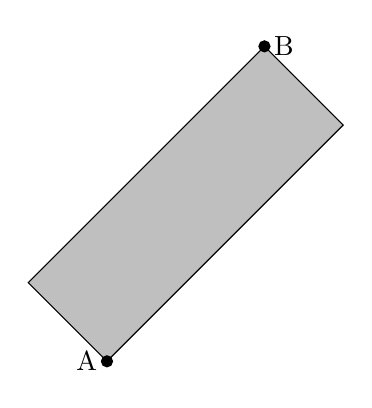
\begin{tikzpicture}
\fill [fill=lightgray] (0,0) -- (-1,1) -- (2,4) -- (3,3) -- cycle;
\draw  [latex-latex](0,0) -- (-1,1) -- (2,4)-- (3,3) -- cycle;

\filldraw (0,0) node[left] {A} circle (2pt);
\filldraw (2,4) node[right]{B} circle (2pt);
\end{tikzpicture}
\end{center}

Drop an altitude from B to line up horizontally with A and label the end-point D.
The length |AD| and |BD| are the coordinates.

\begin{center}
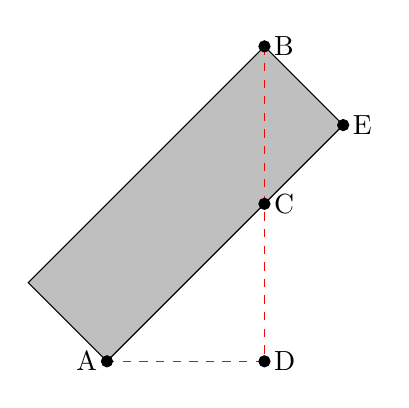
\begin{tikzpicture}
\fill [fill=lightgray] (0,0) -- (-1,1) -- (2,4) -- (3,3) -- cycle;
\draw  [latex-latex](0,0) -- (-1,1) -- (2,4)-- (3,3) -- cycle;

\draw[dashed,red] (2,4)-- (2,2)--(2,0) -- (0,0);

\filldraw (0,0) node[left] {A} circle (2pt);
\filldraw (2,4) node[right]{B} circle (2pt);
\filldraw (2,2) node[right]{C} circle (2pt);
\filldraw (2,0) node[right]{D} circle (2pt);
\filldraw (3,3) node[right]{E} circle (2pt);
\end{tikzpicture}
\end{center}

The triangles $\triangle$ACD and $\triangle$BCE are $45^\circ-90^\circ-45^\circ$ triangles meaning:
\begin{equation*}
\begin{aligned}
	\uline{AC} =& \sqrt{2}\uline{AD} \\
	\uline{BE} =& \frac{1}{\sqrt{2}}\uline{BC} \\
	=& \frac{1}{\sqrt{2}}(\uline{BD}-\uline{CD}) \\
	=& \frac{1}{\sqrt{2}}(\uline{BD}-\uline{AD}) \\
\end{aligned}
\end{equation*}

Hence the (signed) area of the rectangle is:
\begin{equation*}
\begin{aligned}
	\uline{BE}\cdot\uline{AE} =&\uline{BE}\cdot(\uline{AC}+\uline{CE}) \\
	=&(\uline{BD}-\uline{AD})(\uline{BD}+\uline{AD})\\
	=&\uline{BD}^2-\uline{AD}^2\\
\end{aligned}
\end{equation*}

\subsection{Causal Metric}
This construction supplies some intuition for Minkowski Metric.
Since if we interpret the plane as the set of events where the horizontal component is space-like and the vertical is time-like.
The reason the rectangle is at a $45^\circ$ is because that's the maximum speed of propagation.
The rectangle's area is a measure of the amount of events in-between the two.
And the sign of the area is the type of causal connection.
Wether the points are in the way (space-like), or another events are a means by which the earlier effect the later (time-like).

\let\uline\undefined

% Copyright 2023 Kieran W Harvie. All rights reserved.

\section{Quick Summary of Spaces}
A space is a collection of elements, often called points,
with some additional structure.
There are four main types of spaces that form a nice hierarchy,
that is that some types of spaces are always a subtype of other space.
\subsection{Hierarchy}
{\textbf{Topological Space: Neighbourhood}}
In a topological space the elements have a concept of "Neighbourhood",
that is the points which are adjacent to each point.
\begin{center}
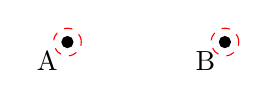
\begin{tikzpicture}
	\draw[dashed,red] (0,0) circle (5pt); 
	\filldraw (0,0) node[below left] {A} circle (2pt);
	\draw[dashed,red] (2,0) circle (5pt); 
	\filldraw (2,0) node[below left] {B} circle (2pt);
\end{tikzpicture}
\end{center}

{\textbf{Metric Space: Distance}}
In a metric space the element have a concept of distance to each other.
You can induce a neighbourhood by saying all points within a certain threshold distance to a point are in the neighbourhood of that point.
\begin{center}
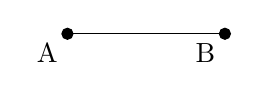
\begin{tikzpicture}
	\draw (0,0) -- (2,0);
	\filldraw (0,0) node[below left] {A} circle (2pt);
	\filldraw (2,0) node[below left] {B} circle (2pt);
\end{tikzpicture}
\end{center}

{\textbf{Normed Space: Length}}
In a normed space there is a concept of length of a point.
Shown here as their distance to some origin.
A distance can be induced by getting the length of an arrow going from A to B.
\begin{center}
\begin{tikzpicture}
	\draw[->] (0,0) -- (0,3.8);
	\draw[->] (0,0) -- (1.9,2.9);
	\filldraw (0,0) node[below] {O} circle (2pt);
	\filldraw (0,4) node[left] {A} circle (2pt);
	\filldraw (2,3) node[right] {B} circle (2pt);
\end{tikzpicture}
\end{center}


{\textbf{Inner-product Space: Projection}}
An inner product space has a concept of projecting one element on another.
You can induce a length by projecting an object onto itself.
\begin{center}
\begin{tikzpicture}
	\draw[->] (0,0) --(0,4.8);
	\draw[->] (0,0) -- (1.9,1.9);
	\draw[red,dashed] (2,2) -- (0,4);
	\draw (1.7,2.3) -- (1.4,2) -- (1.7,1.7);
	\filldraw (0,0) node[below] {O} circle (2pt);
	\filldraw (0,5) node[left] {A} circle (2pt);
	\filldraw (2,2) node[right] {B} circle (2pt);
	\filldraw (0,4) node[left] {B$'$} circle (2pt);
\end{tikzpicture}
\end{center}

\subsection{Euclidean}
Euclidean space is a normed space on $\mathbb{R}^n$ where the inner product is given by $\sum_k A_kB_k$.
This naturally induces a metric on $\mathbb{R}^n$.

The reason we care about the metric of Euclidean space is because all normed spaces have a form of the Pythagorean theorem.
Making metric space the most endowed space we can easily start thinking about non-Euclidean space.

This sucks because most talk about non-Euclidean space talks about "parallel lines" which makes one naturally think about angles and hence an inner product.
But no, instead we have the concept of a geodesic.
A geodesic is a curve that is locally distance minimizing.
This locality comes from the topology, and means that for all points $\gamma(t_1)$ and $\gamma(t_0)$ on the curve $\gamma$ such that they are in the same neighbourhood satisfy:
\[ d(\gamma(t_1),\gamma(t_0)) = k|t_1-t_2|\]

\subsection{non-Euclidean}
Quick rundown of some attempts of non-Euclidean geometries:

Pseudo-Euclidean: Like how we defined Euclidean Space was defined with an inner product we define a new structure with a different quadratic form.
\\

Riemann Manifold: A Manifold is a space that is "locally Euclidean". And a Riemann Manifold is one where this inner-product in the local Euclidean space is always positive.\\

Pseudo-Riemann Manifold: Like A Riemann Manifold but the inner-product is only required to be non-degenerate. I think this includes Pseudo-Euclidean space, but haven't put much thought into it.

%\documentclass[12pt]{article}
%\usepackage{amsmath}
%\usepackage{amssymb}

\section{Wave Equation}
\subsection{Symmetry}
Given some function $u(\vec{x},t)$ on space and time we want to understand it's dynamics under the following assumptions:
\begin{enumerate}
	\item {\textbf{Reversible}}, the dynamics should be symmetric in respect to reversing time.
	\item {\textbf{Isotropic}}, the function should be symmetric in respect to all directions.
	\item {\textbf{Relative}}, the absolute value doesn't matter, only changes.
	\item {\textbf{Perturbation}}, the changes should be small.
\end{enumerate}

The wave equation is a natural conclusion from from these constraints:
\[\frac{\partial^2}{\partial t^2}u = c\sum_i \frac{\partial^2}{\partial x_i^2} u\]

Because the change change is small we start by considering a Taylor expansion and try to get the lowest order terms.
Because it's relative we ignore the $0^\text{th}$ order terms.
Because it's reversible we ignore the $1^\text{st}$ order terms
Giving:
\[\frac{\partial^2}{\partial t^2}u = \sum_{i,j} w_{i,j}\frac{\partial^2}{\partial x_i \partial x_j} u\]
Because it's isotropic all the $\frac{\partial^2}{\partial x_i^2}$ coefficient need to be equal.
And without loss of generality we can assume a basis where the cross terms vanish, giving:
\[\frac{\partial^2}{\partial t^2}u = \sum_i cu\frac{\partial^2}{\partial x_i^2} = c\sum_i \frac{\partial^2}{\partial x_i^2} u\quad \square\]

\subsection{Old Symmetry Attempt}
(Not sure what I was doing here, lol. Seems like I went on the wrong path by not including $t$)
Lets start with with a function of space $u(\vec{x})$.
Lets assume it is continuous such that:
\[u(\vec{x} +\vec{r}) = u(\vec{x}) + \sum_{i}r_i\frac{\partial}{\partial x_i}u(\vec{x})+\frac{1}{2}\sum_{i,j}r_ir_j\frac{\partial^2}{\partial x_i\partial x_j}u(\vec{x}) \]
Lets remove all terms that aren't reversible:
\[u(\vec{x} +\vec{r}) = u(\vec{x}) + \frac{1}{2}\sum_{i}r_i^2\frac{\partial^2}{\partial x_i^2}u(\vec{x}) \]
Lets impose localization:
\[c^2r_0^2 = \sum_{i>0}r_i^2\]
Not sure exactly how this part works but we get the sign we need one example is to only keep terms that have $c^2r_0^2 = r_i^2$

\subsection{1-D}
I need to remind myself how to solve the 1-D case as a stepping stone for something else.
Reminder that the 1-D form, with unitary speed, is:
\[ \frac{\partial^2}{\partial t^2} u = \frac{\partial^2}{\partial x^2}u\]
Observe that plane waves where angular frequency and wave number have the same magnitude solve this:
\[ \exp(ik(x\pm t))\]
This suggests the use of Fourier transform, where the $\pm$ is used to fit the solution to initial value and derivative:
\[ u = \frac{1}{\sqrt{2\pi}}\int_\mathbb{R}(a_+(k)e^{ikt}+a_-(k)e^{-ikt})e^{ikx}\,dk\]
Assume $f(x) = u(x,0)$ and $h(x) = \left[\frac{\partial}{\partial t}u\right](x,0)$.
Equating Fourier transforms gives:
\begin{equation*}
\begin{aligned}
	\hat{f}(k) =& a_+(k)+a_-(k) \\
	\hat{h}(k) =& ik(a_+(k)-a_-(k)) \\
\end{aligned}
\end{equation*}
Hence:
\[ u = \frac{1}{\sqrt{2\pi}}\int_\mathbb{R}(\hat{f}(k)\cos(kt)+\hat{h}(k)k^{-1}\sin(kt))e^{ikx}\,dk\]
\\

This can be processed further through the convolutions theorem.
(Because of the table of transforms I have it will be easier $\sin$ is turned into normalized $\sinc$ and $\rect$ cuts off at $\frac{1}{2}$):
\[ u = \frac{1}{\sqrt{2\pi}}\int_\mathbb{R}\left(\hat{f}(k)\cos(kt)+\hat{h}(k)t\sinc\left(\frac{kt}{\pi}\right)\right)e^{ikx}\,dk\]

\begin{equation*}
\begin{aligned}
	u =& \left[f(\tau)\ast\frac{1}{2}(\delta(\tau-t)+\delta(\tau+t))\right](x) + \frac{\sgn(t)}{2}\left[h(\tau)\ast\rect\left(\frac{\tau}{2t}\right)\right](x)\\
	 =&  \frac{1}{2}(f(x-t)+f(x+t)) + \frac{\sgn(t)}{2}\left[h(\tau)\ast\rect\left(\frac{\tau}{2t}\right)\right](x)\\
	 =&  \frac{1}{2}(f(x-t)+f(x+t)) + \frac{\sgn(t)}{2}\int_{x-t}^{x+t}h(\tau)\,d\tau\\
\end{aligned}
\end{equation*}

Which is such a cool equation!
It shows the reversibility and isotropic nature of the solution but the evenness of $x$ and $t$.
It shows the limit on how fast information travels by the convolution with $\rect$.

I don't really like the $\sgn$ function there and I'm not convinced it isn't some kind of error. 
So ignoring it for the following bit (it's mostly $\pm 1$ anyway),
see how we can recover the conditions on $f$ and $h$:
\begin{equation*}
\begin{aligned}
	u(x,0) =&  \frac{1}{2}(f(x-0)+f(x+0)) + \frac{1}{2}\int_{x-0}^{x+0}h(\tau)\,d\tau \\
	=& f(x) \\
	\left[\frac{\partial}{\partial t}u\right](x,t) =&  \frac{1}{2}-(f(x-t)+f(x+t)) + \frac{1}{2}(h(x-t)+h(x+t)) \\
	\left[\frac{\partial}{\partial t}u\right](x,0) =&  h(x) \\
\end{aligned}
\end{equation*}
It almost seems obvious! 
Like I should have gone straight to this and not bothered with the Fourier stuff.
At least I learn something, I guess.

\section{Unit Fraction}
\textbf{Theorem:}
Consider a function $f:X \rightarrow \mathbb{R}$ where $\cl(\im(f))$ is bounded and countable.
Then for any $n\in\mathbb{N}$ and interval $U\subset \mathbb{R}$ we have $n\im(f) \not\supseteq\mathbb{Q} \cap U$.
\footnote{In this section $nS$ means $\{\sum_i s_i | s\in S^n\}$ and not $\{ns | s\in S\}$} 
\\

\textbf{Proof:}
If we assume that $n\im(f) \supseteq \mathbb{Q} \cap U$ we get:
\[|\cl(n\im(f))| \geq |\cl(\mathbb{Q} \cap U)| = |U| = \aleph_1 \]
However by the compactness of $\cl(\im(f))$:
\[\cl(n\im(f))= n\cl(\im(f))\]
Hence by the countability of $\cl(\im(f))$:
\[|\cl(n\im(f))| = |n \cl(\im(f))| \leq |\cl(\im(f))|^n = \aleph_0^n = \aleph_0\]
This contradicts $|\cl(n\im(f))| \geq \aleph_1$ and hence $n\im(f) \not\supseteq\mathbb{Q} \cap U$.
\\

\textbf{Corollary:}
The function $f:\mathbb{N}_{>0} \rightarrow \mathbb{R}$ where $f(x) = 1/x$ meets the function requirements.
Hence for every interval there is a rational number that can't be represented with $n$ unit fractions.
\\

I want to try a more aesthetically pleasing formulation by separating out the set theory from the topology from the $\mathbb{Q}$ specifics. 
\\

\textbf{Theorem:} Let $X$ and $Y$ be sets. 
Then $|Y| > |X|^n$ implies $nX \not\supseteq Y$.

\textbf{Proof:} By contradiction on set size.
\\

\textbf{Theorem:} If $X$ is countable and $Y$ is non-countable then $nX \not\supseteq Y$ for all $n\in\mathbb{N}_{>0}$.

\textbf{Proof:} The previous theorem using $\aleph_1 > \aleph_0^n$ for all $n\in\mathbb{N}_{>0}$
\\

\textbf{Theorem:} If $X$ is compact, $\cl(X)$ countable, and $Y$ non-countable then $\cl(nX) \not\supseteq Y$ for all $n\in\mathbb{N}_{>0}$.

\textbf{Proof:} The previous theorem using $\cl(nX) = n\cl(X)$ from compactness.
\\

Now just rework the corollary a bit for it to fit here. 

\section{Winquist's identity}
The following form of the Winquist's identity was on an old hard drive:
\begin{equation*}
\begin{aligned}
	\prod_{n \geq 1}&(1-ax^{n-1})(1-a^{-1}x^n)(1-bx^{n-1})(1-b^{-1}x^{n}) \\
	&\times(1-ab^{-1}x^{n-1})(1-abx^{n-1})(1-a^{-1}b^{-1}x^{n})(1-x^n)^2 \\
	=& \sum_{i \in \mathbb{N}_{\geq 0}}\sum_{j\in\mathbb{Z}} (-1)^{i+j}(b^{-3j}-b^{3j+1})(a^{-3i}-a^{3i+3}) \\
	&\times(b^{-3i+2}-b^{3i-1})(a^{-3j+1}-a^{3j+2})x^{\frac{j(3j+1)}{2}+\frac{3i(i+1)}{2}} \\
\end{aligned}
\end{equation*}

A quick Google make the identity verifies that the identity looks right.
With the exception of the ranges of the RHS summation, maybe $i$ and $j$ should be switched.
\\

Either way this is a cool identity and captures something interesting.
And that would definitely be helpful in generating functions.
In particular reciprocating the relation and multiplying by the RHS give a weighted partition that has a relatively sparse recursive relation.

% Copyright 2023 Kieran W Harvie. All rights reserved.

\section{XOR hash}
Today I was presented with the following problem:
\\

Given an array with all integers $[1,100]$ with a single integer removed.
Assuming memory is limited, how do you efficiently determine the missing integer?
\\

The solution is to XOR all the elements of the array together.
Then XOR this with the known value for ALL the numbers between $[1,100]$.
The result will be the missing number.
\\

This problem seemed like a good introduction to hashes, like Zobrist, that XOR a bunch of info together.
The benefit of this approach is that the components can be added/removed by a XOR:
\[h(\{a_0,a_1\}) = h(\{a_0\})\XOR h(\{a_1\})\]

\subsection{Determining the constant}
It turns out its easy to calculate the constant for the original question by hand.
First define $T$ as:
\[T(n) = n \XOR T(n-1),\quad T(1) = 1\]
Then:
\[T(n) = \begin{cases}n&n \mod 4 = 0 \\1& n\mod 4 = 1\\ n+1 &n\mod 4 = 2\\ 0& n\mod 4 = 3\end{cases}\]
This can easily be proved by induction and remembering that for even $n$ we have:
\[n\XOR 1 = n+1\]

Because of the modularity you would expect there to be an expression for $T$ involving powers of the fourth root of unity ($i$): 
\[T(n) = \frac{1}{2} +\frac{1}{2}(1+(-1)^n)+\frac{1}{4}((i-1)(-i)^n-(i+1)i^n)\]
(Done on scrap paper, not double checked, close enough to see the form).
\\

While the hybrid function is probably a more useful form the last one involves complex numbers in a way I didn't expect.

\subsection{Homomorphic Hashing}
Those with mathematic training will notice that the property that make this approach work:
\[h(\{a_0,a_1\}) = h(\{a_0\})\XOR h(\{a_1\})\]
Has the same form as a homomorphism\footnote{"same form" as a "homomorphism", math pun intended} and would investigate homomorphic hash functions. 

Well the most influential definition of such a function happened in 2004 Krohn, Freedman and Mazieres proposed a definition of homomorphic hash function as function $H: V\rightarrow G$ such that:
\begin{itemize}
\item $H$ is collision resistant. Meaning we are unlikely to find $x$ and $y$ such that $H(x) = H(y)$.
\item $H$ is a homomorphism. Meaning $H(x+y) = H(x)+H(y)$ for all $x$ and $y$.
\end{itemize}

The main problem is defining $V$ that is compatible with the regiments on $H$.
Since we want to use the set union operator then the natural choice is $V = 2^S$ for some set $S$.
But our hash only has the same form as a homomorphism\footnote{haha} when the input sets are mutually exclusive.
In general we have:
\[H(S_0 \cup S_1) = H(S_0)\XOR H(S_1) \XOR H(S_0 \cap S_1)\]

We can make a collision resistant hash though.
Make $H$ uniformly distributed on $\mathbb{F}_2^{\log_2|S|}$ for $S$.
Then by induction and $x \XOR y = 0$ iff $x=y$ you can show that it stays uniform for $2^S$.
Meaning the chance of a collision is $\frac{1}{|S|}$

(This is actually a bound for when $|S|$ is a power of $2$, but you can figure out the rest)
\\

Homomorphic functions are still useful in cryptography though.

% Copyright 2023 Kieran W Harvie. All rights reserved.
\section{Rational Tangent}
Consider the following relation:
\begin{equation*}
\begin{aligned}
	\cos(n\phi)+i\sin(n\phi) =& (\cos(\phi)+i\sin(\phi))^{n} \\
	=&(\cos(\phi)(1+i\tan(\phi)))^n\\
	=&\cos(\phi)^n(1+i\tan(\phi))^n\\			
\end{aligned}
\end{equation*}
The product of two complex numbers with rational real and imaginary part is a complex number with rational real and imaginary part.

To see this observe that we only use multiplication, addition, and subtraction to get the real and imaginary components of the product from the component of the factors and that these operations between from rational numbers produce rational numbers.

Hence, if $\tan(\phi)$ is rational the there exists some rational numbers $p,q$ such that:
\[(1+i\tan(\phi))^n = p+qi\]
Substituting this into the original formula:
\[\cos(n\phi)+i\sin(n\phi) = \cos(\phi)^n(p+qi)\]
And equating real and imaginary components gives:
\[\tan(n\phi) = \frac{\sin(n\phi)}{\cos(n\phi)} = \frac{\cos(\phi)^np}{\cos(\phi)^nq} = \frac{p}{q}\]

Hence $\tan(\phi)$ being rational implies $\tan(n\phi)$ is as well.
\\

I think this result was meant to be part of a larger argument,
but I have forgotten what the larger one is.
One point that I think will be relevant is using similar arguments with:
\[\frac{1}{\cos(\phi)+i\sin(\phi)}= \cos(\phi)-i\sin(\phi)\]

\subsection{Brute Force}
Another proof of the same result, 
done by brute force,
was in the same notes on my hard-drive.
Presumably done as a sanity check before figuring out the better method:
\\

$\tan(\phi)$ being rational is the same as saying that $r\sin(\phi) = \cos(\phi)$ for some rational number $r$.
\begin{equation*}
\begin{aligned}
	\sin(n\phi)+i\cos(n\phi) =& \exp(in\phi)\\
	=& \exp(i\phi)^n \\
	=& (\sin(\phi)+i\cos(\phi))^n\\
	=& \sum_{k=0}^{n}\binom{n}{k}i^k\cos(\phi)^k\sin(\phi)^{n-k}\\
	=& \sum_{k=0}^{n}\binom{n}{k}i^kr^k\sin(\phi)^n\\
	=&\sin(\phi)^n\left(\sum_{k=0}^{2k \leq n}\binom{n}{2k}(-1)^kr^{2k}+i\sum_{k=0}^{2k+1 \leq n}\binom{n}{2m+1}(-1)^kr^{2k+1}\right)\\
\end{aligned}
\end{equation*}
Hence:
\[\tan(n\phi) = \frac{\sum_{k=0}^{2k \leq n}\binom{n}{2k}(-1)^kr^{2k}}{\sum_{k=0}^{2k+1 \leq n}\binom{n}{2k+1}(-1)^kr^{2k+1}}\]


% Copyright 2023 Kieran W Harvie. All rights reserved.

\section{Jensen's Inequality}
A convex function $\phi$ on a set $X$ is one such that for $a_n\in X$ with $w_0+w_1 =1$ and $w_n \geq 0$ then we have:
\[\phi(w_0a_0+w_1a_1) \leq w_0\phi(a_0)+w_1\phi(a_1)\]
Jensen's Inequality states that expected value of the function is less then the function of the expected value:
\[\phi(\E(X)) \leq \E(\phi(X))\]

By multiplying the function by $-1$, we get the intuitive corollary that the inequality is reversed for concave functions.

\subsection{Generalization}
A more general form of convexity can be easily proved by induction.
\\

Assume that for some $n$ we have that for all $\sum_{i=1}^nw_i'=1$ and $w_i' \geq 0$:
\[\phi\left(\sum_{i=1}^nw_i'a_i\right) \leq \sum_{i=1}^nw_i'\phi(a_i)\]

Let $\sum_{i=1}^{n+1}w_i=1$ and $W = \sum_{i=1}^nw_i$ we have $w_{n+1}+W = 1$ and :
\begin{equation*}
\begin{aligned}
\phi\left(\sum_{i=1}^{n+1}w_ia_i\right) =&\phi\left(w_{n+1}a_{n+1}+W\sum_{i=1}^{n}\frac{w_i}{W}a_i\right) \\
\leq& w_{n+1}\phi(a_{n+1})+W\phi\left(\sum_{i=1}^{n}\frac{w_i}{W}a_i\right) \\
\leq& w_{n+1}\phi(a_{n+1})+W\sum_{i=1}^n\frac{w_i}{W}\phi(a_i) \\
\leq& \sum_{i=1}^{n+1}w_i\phi(a_i) \\
\end{aligned}
\end{equation*}

Viewing the weights as probabilities this form can directly be in interpreted as a discrete form of Jensen's Inequality.

\subsection{Mean Inequalities}
This can be directly applied to various mean inequalities.
\begin{equation*}
\begin{aligned}
	AM =& \frac{1}{n}\sum_{i=1}^{n}a_i \\
	RMS =& \sqrt{\frac{1}{n}\sum_{i=1}^na_i^2} \\
	GM =& \sqrt[n]{\prod_{i=1}^na_i}\\
\end{aligned}
\end{equation*}
Using $\phi(x)=x^2$,$w_i = \frac{1}{n}$ we directly get:
\[AM^2 \leq RMS^2\]
Using $\phi(x)=\log(x)$,$w_i = \frac{1}{n}$ we get:
\footnote{Remember that the inequality is reversed since $\log$ is concave}
\[\log(AM) \geq \log(GM)\]

Since both these functions are also monotonic the clean relations follow.

\subsection{Decision Theory} 
Interpret $\phi$ as a utility function then the convexity tells us whether we take the fixed $\E(X)$ or risk $X$.
Well if $\phi$ is convex then:
\[\phi(\E(X)) \leq \E(\phi(X))\]
And we should take the risk,
there is more expected utility taking the risk then the utility of $\E(X)$.

If $\phi$ is concave then we should not take the risk.

% Copyright 2023 Kieran W Harvie. All rights reserved.

\section{Convex}
TODO: Flesh out, copy edit, and maybe include pictures for the geometric intuition in the cord section.
\\

In the section of Jensen's Inequality I defined a convex function $\phi$ on a set $X$ as one such that for $a_n\in X$ with $w_0+w_1 =1$ and $w_n \geq 0$ then we have:
\[\phi(w_0a_0+w_1a_1) \leq w_0\phi(a_0)+w_1\phi(a_1)\]
I've thought of another proof of the previous section but iterates over functions instead of points.
And we can use some geometry intuition (cords).
\\

\subsection{Cords}
First let me define a new function called the cord function that takes on an interval $[a,b] \subseteq X$:
\[C_{[a,b]}(x) = \phi(a)+(x-a)\frac{\phi(b)-\phi(a)}{b-a}\]
The convex property can be changed to:
\[x\in [a,b] \Rightarrow \phi(x) \leq C_{[a,b]}(x)\]

{\bf Lemma:}, if $x_0 \leq x_1 \leq x_2$ then:
\[ x\in [x_0,x_1] \Rightarrow C_{[x_0,x_1]}(x) \leq C_{[x_0,x_2]}(x)\]
and:
\[ x\in [x_1,x_2] \Rightarrow C_{[x_1,x_2]}(x) \leq C_{[x_0,x_2]}(x)\]
{\bf Proof:} Use $C_{[a,b]}(a) = \phi(a)$ or $C_{[a,b]}(b) = \phi(b)$ and $x_1 \in [x_0,x_2]$ with the definition of convexity.
\\

{\bf Lemma:}, if $a_0 \leq a_1 \leq b_1 \leq b_0$ then:
\[x\in [a_1,b_1] \Rightarrow C_{[a_1,b_1]}(x) \leq C_{[a_0,b_0]}(x)\]
{\bf Proof:} use the previous lemma with the triples form the quad inequality, then chain together the newer inequalities.
\\

Let:
\[\phi_{[A,B]}(x) = \begin{cases} C_{[A,B]}(x) & x\in [A,B] \\ \phi(x) &\text{else} \end{cases}\]
$\phi_{[A,B]}(x)$ is convex.
Prove this using the previous lemmas with the three cases (points same side, both sides, one in one out).

\subsection{The Cool Proof}
We want to show that for all $\sum_{i=1}^nw_i'=1$ and $w_i' \geq 0$:
\[\phi\left(\sum_{i=1}^nw_i'a_i\right) \leq \sum_{i=1}^nw_i'\phi(a_i)\]

Assume it works for $n-1$ points.
Take two points $(w_0,a_0)$ and $(w_1,a_1)$ and make a new convex function using the method from the previous section with $[x_0,x_1]$, then remove the two points and replace with $(w_0+w_1, \frac{w_0a_1+w_1a_1}{w_1+w_0})$.
Now we have a $n-1$ points,
and if you expand the algebra you get the correct form,
hence by induction you prove the initial result.

% Copyright 2023 Kieran W Harvie. All rights reserved.
\section{Old Geometry}
Bellow are are collection of proofs from high school that I saved under "geometry".
It includes triangle groups and two (half complete) geodesics.
\subsection{Triangle Groups}
Are a way of understanding the rotations of platonic solids.
Fill in latter
\subsubsection{Subgroup chain}
Let:
\[\iota^2 = \lambda^4 = \kappa^3 = 1\]
With and those be the lowest powers that do so.
Additionally have:
\[\lambda = \iota\kappa\]
This is a cube, $\iota$ rotates around a edge, $\kappa$ rotates around a vertex, $\lambda$ rotates around a face.

Let:
\[i = \lambda^2,\,k=\lambda\iota,\,k=\kappa^2\]
We have:
\begin{equation*}
\begin{aligned}
i^2 =& \lambda^4\\
	=& 1 \\
k^3 =& \kappa^6\\
	=&1\\
l^3 =& (\lambda\iota)^3\\
	=&(\iota\kappa\iota)^3\\
	=&\iota\kappa^3\iota\\
	=&1\\
\end{aligned}
\end{equation*}
These are the lowest powers to do so.
Minimality is trivial for $i$ and $k$ by the minimality of $\kappa$ and $\iota$.
For $l$ assume $l^2 = 1$ then:
\begin{equation*}
\begin{aligned}
l^2 =& 1\\
\lambda\iota\lambda\iota =& 1\\
\iota\lambda\iota =& \lambda^3\\
\kappa\iota =& \lambda^3\\
\kappa\iota\lambda =& \lambda^4\\
=&1\\
\kappa^2 =& 1\\
\end{aligned}
\end{equation*}
We have the relation:
\begin{equation*}
\begin{aligned}
ik =& \lambda^3\iota\\
	=&\lambda^3\iota\kappa^3\\
	=&\lambda^3\lambda\kappa^2\\
	=&\kappa^2\\
\end{aligned}
\end{equation*}
Hence the rotations of a regular tetrahedron are a subgroup of the rotations of a cube.
\subsection{Torus}
Let a torus be parametrized by:
\begin{equation*}
\begin{aligned}
	r =&\,(x,y,z) \\
	x =&\, (R+r\cos(\theta))\cos(\phi)\\
	y =&\, (R+r\cos(\theta))\sin(\phi)\\
	z =&\, r\sin(\theta) \\
\end{aligned}
\end{equation*}
The partials of r are given by:
\begin{equation*}
\begin{aligned}
	\frac{\partial r}{\partial \phi} =&\, (-(R+r\cos(\theta))\sin(\phi),(R+r\cos(\theta))\cos(\phi),0) \\
	\frac{\partial r}{\partial \theta} =&\, (-r\sin(\theta)\cos(\phi),-r\sin(\theta)\sin(\phi),r\cos(\theta)) \\
	\frac{\partial r}{\partial \phi}\cdot\frac{\partial r}{\partial \phi} =&\, (R+r\cos(\theta))^2 \\
	\frac{\partial r}{\partial \theta}\cdot\frac{\partial r}{\partial \theta} =&\, r^2 \\
	\frac{\partial r}{\partial \theta}\cdot\frac{\partial r}{\partial \phi} =&\, 0 \\
\end{aligned}
\end{equation*}
Use the partial to get the line element:
\begin{equation*}
\begin{aligned}
	\dot{r}^2 =&\, \left(\frac{\partial r}{\partial \phi}\dot{\phi} + \frac{\partial r}{\partial \theta}\dot{\theta}\right)^2 \\
	=&\, \frac{\partial r}{\partial \phi}\cdot\frac{\partial r}{\partial \phi}\dot{\phi}^2+ \frac{\partial r}{\partial \theta}\cdot\frac{\partial r}{\partial \theta}\dot{\theta}^2+2\frac{\partial r}{\partial \theta}\cdot\frac{\partial r}{\partial \phi} \dot{\phi}\dot{\theta} \\
	=&\, (R+r\cos(\theta))^2\dot{\phi}^2+ r^2\dot{\theta}^2\\
\end{aligned}
\end{equation*}
Treating the line element as the integrand in Lagrangian integral:
\[ L = \frac{1}{2}\dot{r}^2\]
\begin{equation*}
\begin{aligned}
	\frac{\partial L}{\partial \phi} =& \frac{d}{d t}\frac{\partial L}{\partial \dot{\phi}}\\	
	0 =& \frac{d}{d t}(R+r\cos(\theta))^2\dot{\phi} \\
	=& \left[\dot{\theta}\frac{\partial}{\partial \theta} + \ddot{\phi}\frac{\partial}{\partial \dot{\phi}}\right](R+r\cos(\theta))^2\dot{\phi} \\
	=& (R+r\cos(\theta))^2\ddot{\phi}-2r\sin(\theta)(R+r\cos(\theta))\dot{\phi}\dot{\theta} \\
	\ddot{\phi} =& \frac{2r\sin(\theta)}{R+r\cos(\theta)}\dot{\phi}\dot{\theta} \\
\end{aligned}
\end{equation*}
And again:
\begin{equation*}
\begin{aligned}
	\frac{\partial L}{\partial \theta} =& \frac{d}{d t}\frac{\partial L}{\partial \dot{\theta}}\\	
	-r\sin(\theta)(R+r\cos(\theta))\ddot{\phi}^2 =& r^2\frac{d}{dt}\dot{\theta} \\
	-r\sin(\theta)(R+r\cos(\theta))\ddot{\phi}^2 =& r^2\ddot{\theta} \\
\end{aligned}
\end{equation*}
\subsection{Sphere}
Let a sphere be parametrized by:
\begin{equation*}
\begin{aligned}
	r =&\,(x,y,z) \\
	x =&\, \cos(\theta)\cos(\phi)\\
	y =&\, \cos(\theta)\sin(\phi)\\
	z =&\, \sin(\theta) \\
\end{aligned}
\end{equation*}
The partials of r are given by:
\begin{equation*}
\begin{aligned}
	\frac{\partial r}{\partial \phi} =&\,(-\cos(\theta)\sin(\phi),\cos(\theta)\cos(\phi),0)\\
	\frac{\partial r}{\partial \theta} =&\, (-\sin(\theta)\cos(\phi),-\sin(\theta)\sin(\phi),\cos(\theta)) \\
	\frac{\partial r}{\partial \phi}\cdot\frac{\partial r}{\partial \phi} =&\, \cos(\theta)^2 \\
	\frac{\partial r}{\partial \theta}\cdot\frac{\partial r}{\partial \theta} =&\, 1 \\
	\frac{\partial r}{\partial \theta}\cdot\frac{\partial r}{\partial \phi} =&\, 0 \\
\end{aligned}
\end{equation*}
Use the partial to get the line element:
\begin{equation*}
\begin{aligned}
	\dot{r}^2 =&\, \left(\frac{\partial r}{\partial \phi}\dot{\phi} + \frac{\partial r}{\partial \theta}\dot{\theta}\right)^2 \\
	=&\, \frac{\partial r}{\partial \phi}\cdot\frac{\partial r}{\partial \phi}\dot{\phi}^2+ \frac{\partial r}{\partial \theta}\cdot\frac{\partial r}{\partial \theta}\dot{\theta}^2+2\frac{\partial r}{\partial \theta}\cdot\frac{\partial r}{\partial \phi} \dot{\phi}\dot{\theta} \\
	=&\, \cos(\theta)^2\dot{\phi}^2+ \dot{\theta}^2\\
\end{aligned}
\end{equation*}
Geodesic Equations:
\begin{equation*}
\begin{aligned}
	\ddot{\theta} =& -\sin(\theta)\cos(\theta)\dot{\phi}^2\\
	0 =& \frac{d}{dt}\cos(\theta)^2\dot{\phi} \\
	=& \cos(\theta)^2\ddot{\phi}-2\cos(\theta)\sin(\theta)\dot{\phi}\dot{\theta} \\
\end{aligned}
\end{equation*}
Consider the function:
\begin{equation*}
\begin{aligned}
	f(t) =& z + \alpha x + \beta y \\
	f(t) =& \sin(\theta) + \alpha\cos(\theta)\cos(\phi) + \beta\cos(\theta)\sin(\phi) \\
	\dot{f}(t) =& \dot{\theta}\cos(\theta)+\alpha(-\dot{\theta}\sin(\theta)\cos(\phi)-\dot{\phi}\cos(\theta)\sin(\phi)) + \beta(-\dot{\theta}\sin(\theta)\sin(\phi)+\dot{\phi}\cos(\theta)\cos(\phi))\\
\end{aligned}
\end{equation*}

\begin{equation*}
\begin{aligned}
\end{aligned}
\end{equation*}

% Copyright 2023 Kieran W Harvie. All rights reserved.

\section{Isomorphisms of the quotient rings of $\mathbb{Z}[X]$ }
While working elsewhere I thought that it's actually really easy to prove:
\[\gcd(a,d)=\gcd(b,d) \Rightarrow \exists z \in\mathbb{Z} \text{ such that } z\frac{a}{d}-\frac{b}{d} \in \mathbb{Z}\]
Using Bézout's identity.
\\

\subsection{The proof}
From Bézout's identity we know there exits $r,s$ in $\mathbb{Z}$ such that:
\[ra+sd = \gcd(a,d) = \gcd(b,d)\]
From the definition of $\gcd$ there exists $d'\in\mathbb{Z}$ such that:
\[b'\gcd(b,d) = b\]
Multiplying the first equation by $b'$ gives:
\[(rb')a+(sb')d = b'\gcd(b,d) = b\]
Hence:
\[(rb')\frac{a}{d}-b\frac{b}{d} = -(sb')\]
As required.
\\

Note that we can actually control the size, and hence sign, of $z$ by using the:
\[ra+sd = a(r+bk)+b(s-ak)\]
Trick, meaning we can force $z>0$ and hence $z\in\mathbb{N}$.

\subsection{The questions}
So this proof brings up some questions:
\begin{enumerate}
	\item Doesn't this prove that $\mathbb{Z}[X]/(dX-a) \cong \mathbb{Z}[X]/(dX-b)$?
	\item Couldn't this be generalized to Bézout Domains?
	\item What about the converse?
\end{enumerate}

\subsection{Question 1}
Let:
\[A = \mathbb{Z}[X]/(dX-a),\quad B =\mathbb{Z}[X]/(dX-b)\]
We can say $A$ and $B \subset \mathbb{Q}$ where we identity $X$ with $\frac{a}{d}$ and $\frac{b}{d}$ respectfully. 
But since we can find a linear relation between the two $X$s in terms, we need two relations but we can avoid division completely, of the sub-field $\mathbb{Z}$ I'd expect an isomorphism.
\\

Assume the $\gcd$ condition is meet and let $z_0$ and $z_1$ be the integers such that:
\[z_1\frac{a}{d}-\frac{b}{d} = -z_0\]
Equally written as:
\[d(z_1a+z_0)=b\]

\subsubsection{Attempt 1}
Define $\phi: B \rightarrow A$.
A ring homomorphism fixes $1$ and hence acts identically on the set generated by $1$,
that is $\mathbb{Z}$.
Since $a\in\mathbb{Z}$ hence:
\begin{equation*}
\begin{aligned}
	a =& \phi(a) \\
	=&\phi(dX) \\
	=&d\phi(X) \\
\end{aligned}
\end{equation*}
Suggesting a form for $\phi(X)$:
\[\phi(X) = z_1X+z_0\]
This is all the degrees of freedom we get since being a homomorphism requires:
\[\phi\left(\sum_np_nX^n\right) = \sum_n\phi(p_n)\phi(X)^n\]
Hence the suggested form is:
\[\phi\left(\sum_np_nX^n\right) = \sum_np_n(z_1X+z_0)^n\]

But dealing with showing homomorphism when dealing the canceling term isn't something I want to do.

\subsubsection{Attempt 2}
Define a function $\phi: \mathbb{Z}[X] \rightarrow B$ where:
\[\phi\left(\sum_np_nX^n\right) = \sum_np_n(z_1X+z_0)^n\mod (dX-b)\]
Then we can use the first isomorphism theorem of rings and only need to show that $\phi$ is surjective and has a kernel of  $\langle dX-a \rangle$.

% Copyright 2023 Kieran W Harvie. All rights reserved.

\section{Generated Subfield of Finite Fields}
Let the finite field $F$ have a set of elements $S$.
The set $\langle S \rangle$ whose elements are the sums of the products of powers of $S$:
\[\langle S \rangle = \left\{\sum_n\prod_i s_i^{p_{i,n}}\,|\,s_i\in S \text{ and } p_{i,n}\in \mathbb{Z}\right\}\cup\{0\}\]
For example if $S = \{s_0,s_1,s_2\}$ all of the following are elements of $\langle S \rangle$:
\[s_0+s_1+s_2,\quad s_0s_1s_2s_3,\quad 1+s_0+s_1s_2^7+s_0s_1s_2^2\]
(I use the $\langle \cdot \rangle$ notation because this is like generation,
one of the most irregular and abused words in algebra).
\\

The set inherits it's operations from $F$ and is clearly closed under addition and multiplication.
It also contains $1$ and its repeated sum, labeled $n$, by using $p_{i,n} = 0$:
\[n = \overbrace{(s_0s_1s_2)^0+(s_0s_1s_2)^0+\dots s(s_0s_1s_2)^0}^{n \text{ times}}\]

Given $q\in \langle S \rangle$ because there are a finite number of options for $nq$ the pigeonhole principle means there will eventually be $n > m+1$ such that:
\begin{equation*}
\begin{aligned}
nq =& mq\\
(n-m)q =& 0\\
q+(n-m-1)q=& 0\\
\end{aligned}
\end{equation*}
$(n-m-1)q$ which is the additive inverse of $q$.
Because $n-m-1 > 0$ it is an element of $\langle S \rangle$ and since $q$ is also an element by closure so is the inverse.
\\

Likewise for the multiplicative inverse:
\begin{equation*}
\begin{aligned}
q^n=&q^m\\
q\cdot q^{n-m-1}=&1
\end{aligned}
\end{equation*}
Hence $\langle S \rangle$ is a, not necessarily proper, subfield of $F$.

\subsection{$S=\{1\}$}
An important example is when $S=\{1\}$.
Let $n$ be the "lowest"\footnote{Yes I know I haven't defined that properly, but just figure it out.} where the pigeonhole principle whole applies:
\begin{equation*}
\begin{aligned}
	m + (n-m) =& n+(m-m)\\
	=& n \\
	=& m \\
\end{aligned}
\end{equation*}

The minimality\footnote{See previous footnote.} of $n$ makes $n-m$ non-zero making $n$ zero.
Hence $S\cong\mathbb{F}_{n}$.
\\

(This is sloppy even for quick notes)

\subsection{Dreams of a more rigor}
Let $R$ be a ring and let $\phi$ be a function from $\mathbb{Z}$ to $R$ such that:
\[\phi(1)=1_R,\quad \phi(n\pm 1) = \phi(n)\pm \phi(1_R)= \phi(n)\pm 1_R\]
$\phi$ is well-defined as you can find the value for any $n\in\mathbb{Z}$ by induction.
And the function only has one value at each $n$ since you can't change the value by "doubling back" on the induction:
\[\phi((n\pm 1)\mp 1) = \phi(n\pm 1)\mp 1_R = \phi(n)\pm 1_R\mp 1_R = \phi(n)\]

Induction on $n$ shows:
\begin{equation*}
\begin{aligned}
	\phi(n)+\phi(m) =& \phi(n\pm 1)\mp 1 +\phi(m) \\
	=& \phi(n\pm 1)+\phi(m\mp 1) \\
	=& \phi(n\pm 1 + m\mp 1) \\
	=& \phi(n+m) \\
\end{aligned}
\end{equation*}

Which can be used to further prove:
\begin{equation*}
\begin{aligned}
	\phi(n)\phi(m) =&(\phi(n\pm 1)\mp 1)\phi(m) \\
	=&\phi(n\pm 1)\phi(m)\mp\phi(m) \\
	=&\phi((n\pm 1)m)\mp\phi(m) \\
	=&\phi((n\pm 1)m\mp m) \\
	=&\phi(nm)\\
\end{aligned}
\end{equation*}

These identities,
combined $\phi$ being defined with $\phi(1)=1_R$,
shows that $\phi$ is a homomorphism.
\\

Which, 
by the first isomorphisms theorem for rings,
shows that the $\img\phi$ is a subring of $R$ and is isomorphic to $\mathbb{Z}/\ker \phi$.
This formalizes the concept of the $n$th sum of $1_R$,
and lets us manipulate it better.
\\

\textbf{Corollary:} If $R$ is finite then the additive group of $R$ is also finite.
Meaning $1_R$ has an order,
which we label $N$.
In this case $\ker\phi = N\mathbb{Z}$ giving:
\[\img\phi = \frac{\mathbb{Z}}{N\mathbb{Z}}\]
It's really easy to use Bézout's identity on these objects to show which ones are fields.

\subsection{Wedderburn's Little Theorem}
This is similar to Wedderburn's little theorem, 
that all finite domains are fields.
Wedderburn generalizes the subject to domains instead of field and thus has to use $q-q^n = 0$ and some polynomial analysis (Headache).
But reduces the results,
it doesn't discuss closure.
\\

Cool result,
I suggest looking it up.

% Copyright 2023 Kieran W Harvie. All rights reserved.

\section{Dominated Convergence Theorem}
Consider the following sequences of integrals:
\[I_n = \int_0^1\log(t)^2(1-t)^n\,dt\]
It's related to the Harmonic numbers,
which is why it peaked my interest,
but it was presented in context where we wished to understand its asymptotics.
\\

The book answer of expressing it in terms of hypergeometric functions will be skipped,
because it's boring.

\subsection{Cauchy-Schwartz}
\begin{equation*}
\begin{aligned}
\int_0^1\log(t)^2(1-t)^n\,dt \leq& \sqrt{\int_0^1\log^4(t)\,dt\int_0^1(1-t)^{2n}\,dt}\\
=&\sqrt{4! \frac{1}{2n+1}} \rightarrow 0
\end{aligned}
\end{equation*}
Which by the noticing the sign of $I_n$ and application of the sandwich theorem shows that $I_n \rightarrow 0$.

\subsection{Dominated Convergence Theorem}
As suggested by the section name, this is the result I really want to take notes about.
If a sequence of functions $f_n$ pointwise converge to $f$ and are dominated by some integrable function $g$ such that:
\[|f_n(t)| < g(t)\]
We have:
\[\int_S f_n\,d\mu \rightarrow \int_S f\,d\mu\]
Well rewrite the integral as:
\begin{equation*}
\begin{aligned}
\frac{n}{\log(n)^2}\int_0^1\log(t)^2(1-t)^n\,dt 
=& \int_0^1\left(\frac{(\log(nt)-\log(n)}{\log(n)}\right)^2\left(1-\frac{nt}{n}\right)^n\,d\,nt \\
=&\int_0^n\left(\frac{\log(t)}{\log(n)}-1\right)^2\left(1-\frac{t}{n}\right)^n\,dt \\
=& \int_0^\infty\chi_{[0,n]}(t)\left(1-\frac{\log(t)}{\log(n)}\right)^2\left(1-\frac{t}{n}\right)^n\,dt\\
\end{aligned}
\end{equation*}

Set:
\[f_n(t) = \overbrace{\chi_{[0,n]}(t)\left(1-\frac{\log(t)}{\log(n)}\right)^2}^{g_n(x)}\overbrace{\left(1-\frac{t}{n}\right)^n}^{h_n(t)}\]
We have (pointwise):
\[f_n(t) \rightarrow \exp(-t)\]
We also have $h_n(t) \leq \exp(-t)$ and $g_n(t) \leq (1-\log(t))^2$,
meaning:
\[|f_n(t)| \leq (1-\log(t))^2\exp(-t)\]
Giving the desired result
(Assuming we can show the RHS converges, 
which I'm pretty sure we can since near $0$ we have $\int (1-\log(t))^2\,dt = t(\log(t)^2-4\log(t)+5)$ and far away we have $\exp(-t)$).
\[\frac{n}{\log(n)^2}\int_0^\infty\log(t)^2(1-t)^n\,dt \rightarrow \int_0^\infty\exp(-t)\,dt = 1\]

% Copyright 2023 Kieran W Harvie. All rights reserved.

\section{Divisibility of $(p+1)(p-1)$}
It is well known that if $p$ is prime than either $p$ is a divisor of $6$ or has the remainder $1$ or $5$ when divided by $6$.
This can be verified by noting that a remainder of $0$,$2$, or $4$ would make $p$ divisible by $2$ and likewise for $0$ and $3$ for $3$.
\\

A cool corollary I saw today was that $p$ is a divisor of $6$ or $24$ is a divisor of $(p+1)(p-1)$.
This is also verified by cases:

\begin{center}
\begin{tabular}{|c|cccc|}
\hline
	$p\mod 12$&1&5&7&11\\
\hline
	$\gcd(p+1,12)$&2&6&4&12\\
	$\gcd(p-1,12)$&12&4&6&2\\
\hline
\end{tabular}
\end{center}

The converse isn't true.
Since $24\cdot 3 = 72$,
but $(7-1)(7+1) = 48 < 72$ and $(11-1)(11+1) = 120 > 72$.

% Copyright 2023 Kieran W Harvie. All rights reserved.

\section{Matrix Function Evaluation using Cayley-Hamilton}
(This is something I'm 70\% sure I've seen before but I saw it again today).
(Assume the field is $\mathbb{R}$, don't feel like dealing with others).
\\

The Cayley-Hamilton theorem states that a matrix is the root of it's own characteristic equation.
A cool application of this is simplifying the evaluation of (analytic) matrix functions.
\\

Let $M$ be a matrix with characteristic polynomial $p$,
and eigenvalues $\lambda_i$ with multiplicity $m_i$.
Let the analytic function $f$ be given by:
\[f(x) = \sum_{k=0}^\infty f_kx^k\]
Define a new function $r$ that is interpolated on $\lambda_i$ such that:
\[0\leq k< m_i \Rightarrow\left.\frac{d^k f}{d x^k}\right|_{\lambda_i} =\left.\frac{d^k r}{d x^k}\right|_{\lambda_i}\]
This means that for some analytic function $q$ we have:
\[f(x) = q(x)p(x)+r(x)\]

Now convert these analytic functions to analytic matrix functions in the natural way.
From Cayley-Hamilton theorem we have:
\[f(M) = q(M)p(M)+r(M) = r(M)\]

\subsection{Worked Example}
Let $M$ be a $2\times 2$ matrix with two distinct eigenvalues.
Let $f(x) = \exp(tx)$ then:
\[r(x) = (x-\lambda_0)\frac{\exp(t\lambda_1)}{\lambda_1-\lambda_0}+(x-\lambda_1)\frac{\exp(t\lambda_0)}{\lambda_0-\lambda_1}\]
Hence:
\[f(M) = r(M) =(M-\lambda_0)\frac{\exp(t\lambda_1)}{\lambda_1-\lambda_0}+(M-\lambda_1)\frac{\exp(t\lambda_0)}{\lambda_0-\lambda_1} \]

\subsection{Original Application}
The original problem was to minimize:
\[f(X) = \sum_{k=0}^n\left|\left|\exp\left(\frac{2\pi}{k}B\right)A-X\right|\right|^2\]

Through some procedure similar to the above reasoning it was obtained:
\[\exp(\alpha B) = I+ \sin(\alpha)B+(1-\cos(\alpha))B^2\]

Hence:
\begin{equation*}
\begin{aligned}
&\sum_{k=0}^n\left|\left|\exp\left(\frac{2\pi}{k}B\right)A-X\right|\right|^2\\
=&\sum_{k=0}^n\left|\left|\left(I+\sin\left(\frac{2\pi}{k}\right)B+\left(1-\cos\left(\frac{2\pi}{k}\right)\right)B^2\right)A-X\right|\right|^2\\
=&\sum_{k=0}^n\left|\left|\bigg((I+B^2)A-X\bigg)+\left(\sin\left(\frac{2\pi}{k}\right)B+\cos\left(\frac{2\pi}{k}\right)B^2\right)A\right|\right|^2\\
\end{aligned}
\end{equation*}
The left term independent of $k$ and the right term is independent of $X$.
This means each term of the sum is minimized at:
\[X=(I+B^2)A\]
And since each term is minimized so is the whole sum.

% Copyright 2023-2024 Kieran W Harvie. All rights reserved.

\section{Simplicial Homology}
I need to revise Simplicial Homology so I'm going to give some definitions and then work some examples.

\subsection{Simplicial Definitions}

\subsubsection{Simplex:}
A simplex is a generalization of a triangle to higher/lower dimensions:

\begin{itemize}
	\item 0-simplex is a point
	\item 1-simplex is a segment
	\item 2-simplex is a triangle
	\item 3-simplex is a tetrahedron
\end{itemize}

For our purposes we specify a simplex with an ordered word written from the set of points.
For example $a$ is a point, $bc$ is a segment, and $abc$ is a triangle:
\begin{center}
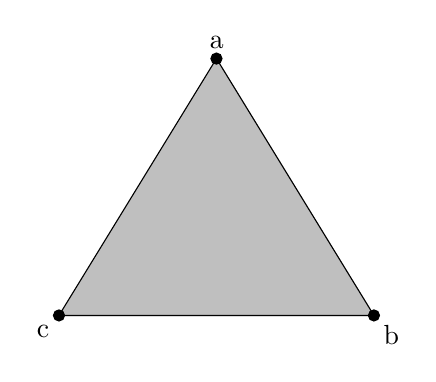
\begin{tikzpicture}
	\filldraw[lightgray] (-2,0)  --(2,0)--(0,3.26210161512);
	\draw (-2,0)--(2,0)--(0,3.26210161512)--(-2,0);
	\filldraw (-2,0) node[below left] {c} circle (2pt);
	\filldraw (2,0) node[below right] {b} circle (2pt);
	\filldraw (0,3.26210161512) node[above] {a} circle (2pt);
\end{tikzpicture}
\end{center}
Two important remarks.
Firstly, $abc\neq acb$ the former one goes around counter-clockwise and the later clockwise.
Secondly, the set $\{ab,bc,bc\}$ is not a triangle and is not the same as $abc$ or $\{abc\}$.
It's all the edges of a triangle but not its interior.

\subsubsection{Face:}
$n$ 0-simplexes defines a $n$-simplex and is called the face of the points.
Conversely the vertices that define a simplex and all the faces that come from that simplex are called the faces of the original simplex.

\subsubsection{Geometric Simplicial Complex}
A Geometric Simplicial Complex $\mathcal{K}$ is a set of simplexes such that:
\begin{enumerate}
	\item Every face of an element of $\mathcal{K}$ is also an element of $\mathcal{K}$.
	\item The non-empty intersection of two simplexes $\sigma_0,\,\sigma_1\in\mathcal{K}$ is a face of both $\sigma_1$ and $\sigma_0$.
\end{enumerate}

\subsubsection{Chain}
A $k$-chain of $\mathcal{K}$ is a formal linear sum of $k$-simplexes.
A $2$-chain is naturally interpreted as a,
possible disconnected and repeated, 
path through $\mathcal{K}$.
\\

More formally, 
given a complex $\mathcal{K}$ the group of $n$-chain $C_n(\mathcal{K})$ is a free $\mathbb{Z}$-module over the $n$-simplexes where two simplexes are equal if they have the same orientation\footnote{The words are even permutation of each other.} and additive inverse if opposite.
(Define $C_{-1} = 0$ for convenience).
\\

For example: $ab+bc$ is the path from $a$ to $c$ through $b$,
$abc = -acb$ are the same triangle with different handedness,
$2ab+dc$ is going over $ab$ twice then jumping to $dc$.
\\

Although the lower dimensions have intuitive geometric interpretation the whole configuration can more intuitively viewed as a combinatoric exercise. 

\subsection{Homology Definitions}
\subsubsection{Boundary Operator}
Given a simplex $\sigma$ define $\sigma_k$ as the same word a $\sigma$ with the $k^\text{th}$ point removed.
The boundary operator $\partial_k:C_k\rightarrow C_{k-1}$ is defined as:
\[\partial_k(\sigma) = \sum_{i=0}^k(-1)^i\sigma_i\]
The boundary of a $0$-simplex is $0$,
the boundary of a $1$-simplex is final point minus inital,
the boundary of a $2$-simplex is it's normal boundary (hence the name).
\\

\begin{equation*}
\begin{aligned}
	\partial_0(a) &= 0\\
	\partial_1(ab) &= b-a\\
	\partial_2(abc) &= ac + cb + bc\\
\end{aligned}
\end{equation*}

\subsubsection{Cycles Subgroup}
The cycles subgroup, $Z_n$, of $C_n$ is the kernel of $\partial_n$:
\[ Z_n = \ker\partial_n\]

The name comes from the $n=1$ case where a $x\in\ker\partial_n$ iff the $1$-chain is cyclic path.

\subsubsection{Boundaries Subgroup}
The boundaries subgroup, $B_n$, of $C_n$ is the image of $\partial_{n+1}$:
\[ B_n = \img\partial_{n+1}\]

The name comes from the $n=1$ case where $\partial_2(x)$ is a $1$-chain going over the boundary of $x$.

\subsubsection{Homology Group}
The boundary of a boundary is $0$.
For intuition consider the $n=1$ case,
the boundary is a cyclic path and hence the boundary of a boundary is zero.
\\

In the general case the boundary of the boundary of $\sigma$ is a sum of words of $\sigma$ with two letters removed where each word appears twice,
once for when the earlier letter is removed first then the last and again in the opposite order.
Let $\sigma_{i,j}$ be the word obtained removing the $i^\text{th}$ and $j^\text{th}$ letter.

When $i< j$ we have:
\[\sigma_{i,j} = (\sigma_i)_j\]
Since taking $i^\text{th}$ out first doesn't effect removing $j^\text{th}$.
And when taking the $j^\text{th}$ element first means the $i^\text{th}$ element is now one letter over:
\[\sigma_{i,j} = (\sigma_j)_{i-1}\]

Now observe that for the sum for the boundary of th boundary:
\begin{equation*}
\begin{aligned}
	\partial_k(\partial_{k+1}(\sigma)) =& \sum_{i=0}^{k}(-1)^i\sum_{j=0}^{k+1}(-1)^j(\sigma_j)_i\\
	=& \sum_{i=0}^{k}\sum_{j=0}^{k+1}(-1)^{i+j}(\sigma_j)_i\\
\end{aligned}
\end{equation*}
Meaning the $j-1$ in the index of the $j$ first case changes the sign of $\sigma_{i,j}$ compared to the $i$ first case.
Hence the terms cancel and the sum is zero.
\\

A direct consequence is that $\img\partial_{n+1}$ is a normal subgroup of $\ker\partial_n$ meaning we can use the fundamental isomorphism theorem to define the quotient group:
\[H_n(\mathcal{K}) = \frac{Z_n}{B_n} = \frac{\ker\partial_n}{\img\partial_{n+1}}\]

\subsection{Worked Examples}
\subsubsection{Disconnected example}
\begin{center}
\begin{tikzpicture}
	\draw (2,0)--(0,3.26210161512);
	\filldraw (-2,0) node[below left] {c} circle (2pt);
	\filldraw (2,0) node[below right] {b} circle (2pt);
	\filldraw (0,3.26210161512) node[above] {a} circle (2pt);
\end{tikzpicture}
\end{center}
\[\mathcal{K}=\{a,b,c,ab\}\]
There's no simplexes of dimensions larger than $3$ hence $C_{n\geq 3} = 0$ and $H_{n\geq 2}(\mathcal{K}) = 0$.
Hence we have:
\[0 \stackrel{\partial_2}{\longrightarrow} C_1 \stackrel{\partial_1}{\longrightarrow} C_0 \stackrel{\partial_0}{\longrightarrow} 0\]
Where:
\[C_1 = \langle ab \rangle,\quad C_0 = \langle a,b,c \rangle\]
All results are pretty trivial:
\begin{equation*}
\begin{aligned}
	&\img \partial_2 = 0 && \ker \partial_1 = 0\\
	&\img \partial_1 = \langle a-b\rangle && \ker \partial_0 = \langle a,b,c\rangle\\
\end{aligned}
\end{equation*}
Gives the homologies:
\begin{equation*}
\begin{aligned}
	H_0(\mathcal{K}) =& \frac{\ker\partial_0}{\img\partial_1} = \frac{\langle a,b,c\rangle}{\langle a-b\rangle} = \langle a,c\rangle = \mathbb{Z}^2\\
	H_1(\mathcal{K}) =& \frac{\ker\partial_1}{\img\partial_2} = 0 \\
\end{aligned}
\end{equation*}


\subsubsection{Triangle without Interior}
\begin{center}
\begin{tikzpicture}
	\draw (-2,0)--(2,0)--(0,3.26210161512)--(-2,0);
	\filldraw (-2,0) node[below left] {c} circle (2pt);
	\filldraw (2,0) node[below right] {b} circle (2pt);
	\filldraw (0,3.26210161512) node[above] {a} circle (2pt);
\end{tikzpicture}
\end{center}
\[\mathcal{K}=\{a,b,c,ab,ac,bc\}\]

Like with the previous example $H_{n\geq 2}(\mathcal{K}) = 0$.
Hence we have:
\[0 \stackrel{\partial_2}{\longrightarrow} C_1 \stackrel{\partial_1}{\longrightarrow} C_0 \stackrel{\partial_0}{\longrightarrow} 0\]
Where:
\[C_1 = \langle ab,ac,bc \rangle,\quad C_0 = \langle a,b,c \rangle\]
The $\ker$ and $\img$ are given bellow:
\begin{equation*}
\begin{aligned}
	&\img \partial_2 = 0 && \ker \partial_1 = \langle ab+bc+ca\rangle\\
	&\img \partial_1 = \langle a-b,a-c,b-c\rangle && \ker \partial_0 = \langle a,b,c\rangle\\
\end{aligned}
\end{equation*}

Proof for $\ker \partial_1$
\begin{equation*}
\begin{aligned}
	&\partial_1(\alpha\,ab+\beta\,bc+\gamma\,ca)\\
	=&\alpha(a-b)+\beta(b-c)+\gamma(c-a) \\
	=&(\alpha-\gamma)a+(-\alpha+\beta)b+(-\beta + \gamma)c \\
\end{aligned}
\end{equation*}
It might already be intuative that you can only choose one of $\alpha,\beta,\gamma$ then the rest are fixed.
But you can also use the following module equation:
\[
	\begin{bmatrix}
		1&0&-1\\
		-1&1&0\\
		0&-1&1\\
	\end{bmatrix}
	\begin{bmatrix}
		\alpha\\
		\beta\\
		\gamma\\
	\end{bmatrix}
	=
	\begin{bmatrix}
		0\\0\\0\\
	\end{bmatrix}
\]

Gives the homologies:
\begin{equation*}
\begin{aligned}
	H_0(\mathcal{K}) =& \frac{\ker\partial_0}{\img\partial_1} = \frac{\langle a,b,c\rangle}{\langle a-b,a-c,b-c\rangle} = \langle a\rangle = \mathbb{Z}\\
	H_1(\mathcal{K}) =& \frac{\ker\partial_1}{\img\partial_2} = \frac{\langle ab+bc+ca\rangle}{0} =\langle ab+bc+ca\rangle =\mathbb{Z}\\
\end{aligned}
\end{equation*}

\subsubsection{Triangle with Interior}
\begin{center}
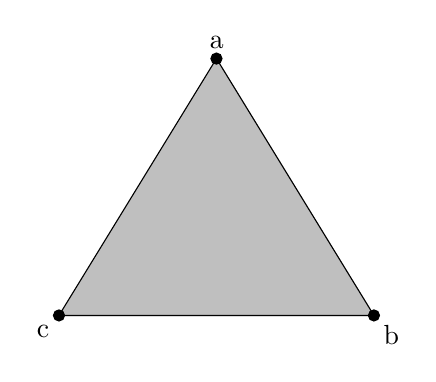
\begin{tikzpicture}
	\filldraw[lightgray] (-2,0)--(2,0)--(0,3.26210161512);
	\draw (-2,0)--(2,0)--(0,3.26210161512)--(-2,0);
	\filldraw (-2,0) node[below left] {c} circle (2pt);
	\filldraw (2,0) node[below right] {b} circle (2pt);
	\filldraw (0,3.26210161512) node[above] {a} circle (2pt);
\end{tikzpicture}
\end{center}
\[\mathcal{K}=\{a,b,c,ab,ac,bc,abc\}\]

There are no simplexes with order larger than $3$ hence like in previous examples $H_{n\geq 3}(\mathcal{K}) = 0$.
Hence we have:
\[0 \stackrel{\partial_3}{\longrightarrow} C_2 \stackrel{\partial_2}{\longrightarrow} C_1 \stackrel{\partial_1}{\longrightarrow} C_0 \stackrel{\partial_0}{\longrightarrow} 0\]
Where:
\[C_2 = \langle abc \rangle,\quad C_1 = \langle ab,ac,bc \rangle,\quad C_0 = \langle a,b,c \rangle\]
The $\ker$ and $\img$ are given bellow:
\begin{equation*}
\begin{aligned}
	&\img \partial_3 = 0 && \ker \partial_2 = 0\\
	&\img \partial_2 = \langle ab+bc+ca\rangle && \ker \partial_1 = \langle ab+bc+ca\rangle\\
	&\img \partial_1 = \langle a-b,a-c,b-c\rangle && \ker \partial_0 = \langle a,b,c\rangle\\
\end{aligned}
\end{equation*}

Gives the homologies:
\begin{equation*}
\begin{aligned}
	H_0(\mathcal{K}) =& \frac{\ker\partial_0}{\img\partial_1} = \frac{\langle a,b,c\rangle}{\langle a-b,a-c,b-c\rangle} = \langle a\rangle = \mathbb{Z}\\
	H_1(\mathcal{K}) =& \frac{\ker\partial_1}{\img\partial_2} = \frac{\langle ab+bc+ca\rangle}{\langle ab+bc+ca\rangle} = 0\\
	H_2(\mathcal{K}) =& \frac{\ker\partial_2}{\img\partial_3} = \frac{0}{0} = 0\\
\end{aligned}
\end{equation*}

\subsection{More Worked Examples}
\subsubsection{Tetrahedron without interior:}
\begin{center}
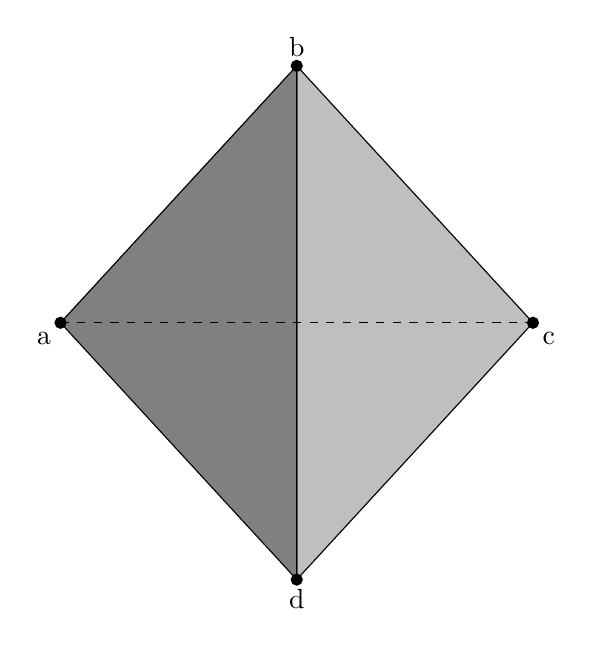
\begin{tikzpicture}
	\filldraw[gray] (-3,0)--(0,3.26210161512)--(0,-3.26210161512);
	\filldraw[lightgray] (0,3.26210161512)--(3,0)--(0,-3.26210161512);
	\draw (-3,0)--(0,3.26210161512)--(0,-3.26210161512)--(-3,0);
	\draw (3,0)--(0,3.26210161512)--(0,-3.26210161512)--(3,0);
	\draw[dashed] (-3,0)--(3,0);
	\filldraw (-3,0) node[below left] {a} circle (2pt);
	\filldraw (0,3.26210161512) node[above] {b} circle (2pt);
	\filldraw (0,-3.26210161512) node[below] {d} circle (2pt);
	\filldraw (3,0) node[below right] {c} circle (2pt);
\end{tikzpicture}
\end{center}
\[\mathcal{K}=\{a,b,c,d,ab,ac,ad,bc,cd,db,abc,abd,acd,cdb\}\]

We have:
\[0 \stackrel{\partial_3}{\longrightarrow} C_2 \stackrel{\partial_2}{\longrightarrow} C_1 \stackrel{\partial_1}{\longrightarrow} C_0 \stackrel{\partial_0}{\longrightarrow} 0\]
Where:
\[C_2 = \langle abc,abd,acd,cbd \rangle,\quad C_1 = \langle ab,ac,ad,bc,bd,dc, \rangle,\quad C_0 = \langle a,b,c \rangle\]
The $\ker$ and $\img$ are larger than previous examples,
despite being simplified,
and are given bellow:
\begin{equation*}
\begin{aligned}
	\img \partial_3 &= 0 \\
	\img \partial_2 &= \langle ab+bc+ca,ab+bd+da,ac+cd+da\rangle\\ 
	\img \partial_1 &= \langle a-b,a-c,a-d\rangle\\
	\ker \partial_2 &= \langle abc+adb+adc+dcb\rangle\\
	\ker \partial_1 &= \langle ab+bc+ca,ab+bd+da,ac+cd+da\rangle\\
	\ker \partial_0 &= \langle a,b,c,d\rangle\\
\end{aligned}
\end{equation*}

Gives the homologies:
\begin{equation*}
\begin{aligned}
	H_0(\mathcal{K}) =& \frac{\ker\partial_0}{\img\partial_1} = \frac{\langle a,b,c,d\rangle}{\langle a-b,a-c,a-d\rangle} = \mathbb{Z}\\
	H_1(\mathcal{K}) =& \frac{\ker\partial_1}{\img\partial_2} = \frac{\langle ab+bc+ca,ab+bd+da,ac+cd+da\rangle}{\langle ab+bc+ca,ab+bd+da,ac+cd+da\rangle} = 0\\
	H_2(\mathcal{K}) =& \frac{\ker\partial_2}{\img\partial_3} = \frac{\langle abc+adb+adc+dcb\rangle}{0} = \mathbb{Z}\\
\end{aligned}
\end{equation*}

\subsubsection{Mixed}
\begin{center}
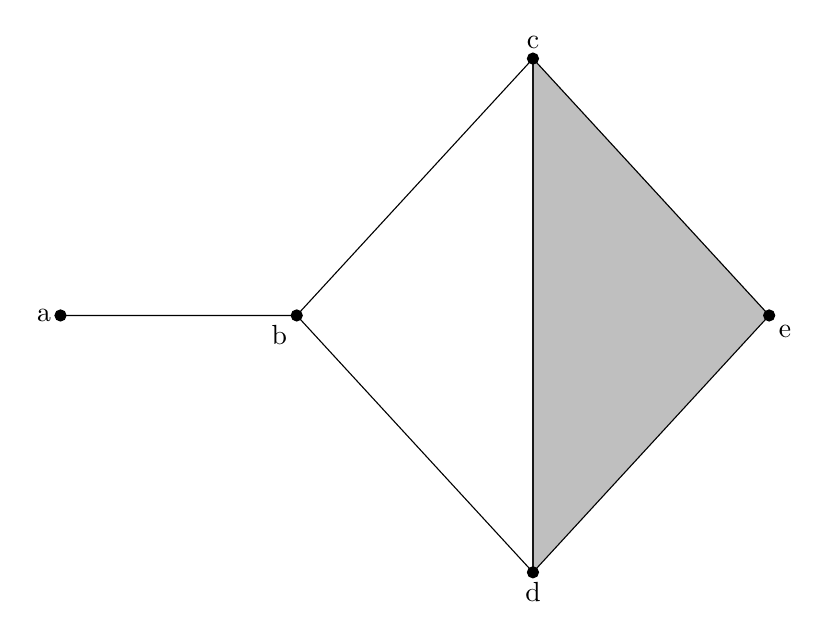
\begin{tikzpicture}
	\filldraw[lightgray] (3,0)--(0,3.26210161512)--(0,-3.26210161512);
	\draw (-6,0)--(-3,0)--(0,3.26210161512)--(0,-3.26210161512)--(-3,0);
	\draw (3,0)--(0,3.26210161512)--(0,-3.26210161512)--(3,0);
	\filldraw (-6,0) node[left] {a} circle (2pt);
	\filldraw (-3,0) node[below left] {b} circle (2pt);
	\filldraw (0,3.26210161512) node[above] {c} circle (2pt);
	\filldraw (0,-3.26210161512) node[below] {d} circle (2pt);
	\filldraw (3,0) node[below right] {e} circle (2pt);
\end{tikzpicture}
\end{center}
\[\mathcal{K}=\{a,b,c,d,e,ab,bc,bd,cd,ec,de,cde\}\]

We have:
\[0 \stackrel{\partial_3}{\longrightarrow} C_2 \stackrel{\partial_2}{\longrightarrow} C_1 \stackrel{\partial_1}{\longrightarrow} C_0 \stackrel{\partial_0}{\longrightarrow} 0\]
Where:
\[C_2 = \langle cde \rangle,\quad C_1 = \langle ab,bc,bd,cd,ec,de \rangle,\quad C_0 = \langle a,b,c,d,e \rangle\]
The $\ker$ and $\img$ are given bellow:
\begin{equation*}
\begin{aligned}
	&\img \partial_3 = 0 && \ker \partial_2 = 0\\
	&\img \partial_2 = \langle ce+ed+dc\rangle && \ker \partial_1 = \langle bc+cd+db, ce+ed+dc\rangle\\
	&\img \partial_1 = \langle a-b,b-c,b-d,c-d,e-c,d-e \rangle && \ker \partial_0 = \langle a,b,c,d,e\rangle\\
\end{aligned}
\end{equation*}

Gives the homologies:
\begin{equation*}
\begin{aligned}
	H_0(\mathcal{K}) =& \frac{\ker\partial_0}{\img\partial_1} = \frac{\langle a,b,c,d,e\rangle}{\langle a-b,b-c,b-d,c-d,e-c,d-e\rangle} = \langle a\rangle = \mathbb{Z}\\
	H_1(\mathcal{K}) =& \frac{\ker\partial_1}{\img\partial_2} = \frac{\langle bc+cd+db,ce+ed+dc\rangle}{\langle ce+ed+dc\rangle} = \langle bc+cd+db\rangle = \mathbb{Z}\\
	H_2(\mathcal{K}) =& \frac{\ker\partial_2}{\img\partial_3} = \frac{0}{0} = 0\\
\end{aligned}
\end{equation*}

\subsection{Interpretation of Simplicial Homology}
Let us summarise the worked example results:
\begin{center}
\begin{tabular}{|c|cccc|}
	\hline
	Complex & $H_0$ & $H_1$ & $H_2$ & $H_{n\geq 3}$ \\ 
	\hline
	Disconnected& $\mathbb{Z}^2$ &0&0&0 \\
	Triangle without interior& $\mathbb{Z}$ & $\mathbb{Z}$ & 0 & 0 \\
	Triangle with interior& $\mathbb{Z}$ & $0$ & 0 & 0 \\
	\hline
	\hline
	Tetrahedron without interior&$\mathbb{Z}$&0&$\mathbb{Z}$&0\\
	Mixed&$\mathbb{Z}$&$\mathbb{Z}$&0&0\\
	\hline
\end{tabular}
\end{center}
But what do they mean?
In a nutshell the power of $\mathbb{Z}$ corresponds to a specific topological feature called an $n$-hole.
A $0$-hole is a connected part,
a $1$-hole is a regular hole,
a $2$-hole is a cavity.
Hence the disconnected complex is made from two connected parts and the rest of one connected part.
And the triangle without an interior has a hole and the others don't.
\\

But why powers of  $\mathbb{Z}$?
And why does $\ker\partial_n / \img\partial_{n+1}$ give this result?
\\

The rigorous answer has to do with homotopy,
and the "Fundamental Homotopy Group" in particular,
which is the math of drawing loops on things then pulling them and then seeing where they get stuck.
Well worth a read but the basics are this:

For every hole you can wrap a loop around it multiple times and in both directions.
Wrapping it around clockwise once is identified with $1$,
wrapping it around counter-clockwise twice is identified with $-2$,
wrapping it around no hole is identified with $0$ since when the loop is pulled taut nothing gets stuck.

If there are two hole $a$ and $b$ then the loops are identified with an element over the free $\mathbb{Z}$-module over $\{a,b\}$.
For example $a+2b$ a clockwise loop over $a$ then two over $b$ and you can add two elements by making a cut in both loops then gluing them together (making sure you preserve orientation).

\begin{center}
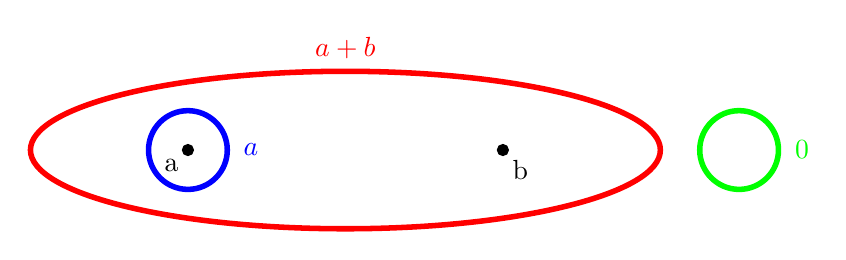
\begin{tikzpicture}
	\filldraw (-2,0) node[below left] {a} circle (2pt);
	\filldraw (2,0) node[below right] {b} circle (2pt);
	\draw[blue,line width=2pt] (-2,0) circle  [radius = 0.5cm];
	\draw[green,line width=2pt] (5,0) circle  [radius = 0.5cm];
	\draw[red,line width=2pt] (0,0) circle [x radius =4cm, y radius = 1cm];
	\node[blue] at (-1.2,0) {$a$};
	\node[green] at (5.8,0) {$0$};
	\node[red] at (0,1.3) {$a+b$};
\end{tikzpicture}
\end{center}

The free $\mathbb{Z}$-module over $\{a,b\}$ is isomorphic to $\mathbb{Z}^2$ because you need two integers to explain all the loops you can make over two holes that stay when taut,
which explains where the powers of $\mathbb{Z}$ came from.

$\ker\partial_n / \img\partial_{n+1}$ works because as noted in the definition of the chain group the elements of the chain group can jump around a bit.
But the requirement $\sigma\in\ker\partial_n$ makes it loop since it's boundary vanishes.
And $\img\partial_{n+1}$ are all the loops that have a higher order faces enabling a taut loop to move freely.
These steps combined give:
\begin{enumerate}
	\item $C_n$ contains all the loops but also completely broken path.
	\item Use $\ker\partial_n$ to get all elements of $C_n$ that are loops.
	\item Modulo $\img\partial_{n+1}$ to remove all loops that don't exit when pulled taut.
\end{enumerate}
\mbox 
Again, this explanation can be made more rigorous by studying homotopy.

\subsection{Boundaries and Cycles}
This is actually obvious,
but applying fundamental isomorphism theorem to $\partial_n:C_n\rightarrow C_{n-1}$ gives:
\[ B_{n-1} = \img\partial_n\cong \frac{C_n}{\ker\partial_n} = \frac{C_n}{Z_n} \]
This gives a new way to interpret $B_n$ based on $Z_n$,
and for $Z_n$ we only need to interpret $\sum_i (-1)^i\sigma_i =0$.
\\

It also makes me aware of how messy boundaries can be\footnote{And in math as well!}.
For example $\{ab,bc\}\subseteq C_1$ means $2a-b-c$ is and element of $B_0$ since you can take a chain of the edge from $b$ to $a$ and $c$ to $a$.

% Copyright 2023 Kieran W Harvie. All rights reserved.

\section{Bounds of Three Series}
Even though I'm sick I found an interesting problem on the internet.
Given positive $a_1,b_1,c_1>0$ and:
\begin{equation*}
\begin{aligned}
	a_{n+1} =& b_n+\frac{1}{c_n}\\
	b_{n+1} =& c_n+\frac{1}{a_n}\\
	c_{n+1} =& a_n+\frac{1}{b_n}\\
\end{aligned}
\end{equation*}

Show that at least one of $a_{800},b_{800},c_{800}$ is greater than 40 and that all sequences are unbounded.

\subsection{Lemma: Closed form for $x_{n+1} = x_n+\frac{k}{x_n}$} 
The closed form is this:
\[ x_{n+1}^2 = x_1^2+2nk+k^2\sum_{l=1}^n\frac{1}{x_l^2}\]
This result is nothing special, 
just a lot of algebra,
the plan is to first get a result for the product of successive terms,
then get perform induction on the product,
and finally cleanup to get the final form.

\begin{equation*}
\begin{aligned}
	x_{n+2}x_{n+1} =& \left(x_{n+1}+\frac{k}{x_{n+1}}\right)x_{n+1}\\
	=& \left(x_n+\frac{k}{x_n}+\frac{k}{x_{n+1}}\right)x_{n+1}\\
	=& x_{n+1}x_n + k +k\frac{x_{n+1}}{x_n} \\
	=& x_{n+1}x_n + k +k\frac{1}{x_n}\left(x_n+\frac{k}{x_n}\right) \\
	=& x_{n+1}x_n + 2k +\frac{k^2}{x_n^2} \\
\end{aligned}
\end{equation*}

Induction gives:
\[ x_{n+2}x_{n+1} = x_2x_1+2nk+k^2\sum_{l=1}^n\frac{1}{x_l^2}\]

Then you clean up by using the initial relation on $x_{n+2}$ and $x_2$.

\subsection{Unbounded:}
Let $s_n = a_n+b_n+c_n$, 
from the HM-AM inequality we have:
\[\frac{1}{a_n}+\frac{1}{b_n}+\frac{1}{c_n} \geq \frac{9}{s_n}\]
With equality if and only if $a_n=b_n=c_n$.
\\

From the series definition we have:
\[s_{n+1} = s_n + \frac{1}{a_n}+\frac{1}{b_n}+\frac{1}{c_n} \geq s_n+\frac{9}{s_n}\]

Since $a_n=b_n=c_n \Rightarrow a_{n+1}=b_{n+1}=c_{n+1}$ we have $s_n$ is bounded by:
\[ s_{n+1}^2 \geq s_1^2+18n+81\sum_{l=1}^n\frac{1}{s_l^2}\]
Hence $s_n$ grows at least as much as $3\sqrt{2n}$,
which is unbounded.
\\

If the sum is unbounded at least one of the series is unbounded.
And if at least one series is unbounded the "swapping" nature of the series means that they all are.

\subsection{$800^\text{th}$ terms:}
Consider the bound sum:
\[ s_{n+1}^2 \geq s_1^2+18n+81\sum_{l=1}^n\frac{1}{s_l^2}\]
If $s_n \leq 1$ then $s_{n+1} > 1$ hence at least half of the time $\frac{1}{s_l^2}$ must be greater than one.
Giving the new bound:
\[ s_{n+1}^2 > 18n+81\left\lfloor\frac{n}{2}\right\rfloor\]
(This isn't a particularly good bound, we could consider $s_1$ separately, but if works the result we need)
Substituting in $n=799$ gives:
\[s_{800}^2 > 18\times799+81\times398 > 18\times800 = 3^2\times40^2\]
Hence:
\[a_{800}+b_{800}+c_{800} = s_{800} > 3\times40\]
From pigeon holing at least one LHS term is greater than 40.

\subsection{Remarks}
This is yet another example of this Olympian style problem where I had to be prompted to consider the HM-AM inequality.

Although I was working with inequalities between elementary polynomial sums so wasn't that far away myself,
and the other advice that was given was just straight up wrong, 
so I should probably just remember to use the inequality means in the future and let it go.

% Copyright 2023 Kieran W Harvie. All rights reserved.

\section{Summation by Parts}
During a boring meeting I was reminded of a cool trick called "Summation by Parts".
Given two sequences $a_n$ and $b_n$ define $B_n = \sum_{k=0}^nb_n$.
Then we have:
\[\sum_{k=0}^Na_nb_n = a_NB_N-\sum_{n=0}^{N-1}B_n(a_{n+1}-a_n)\]
The name is clearly in reference to it being the discrete counterpart to integration by parts.
With integration replaced with summation and derivatives with difference.
\\

I will not be proving this formula, 
doing so is simple algebra.

\subsection{Nicomachus's Theorem}
Nicomachus's Theorem is the name of the following identity:
\[\sum_{k=1}^nk^3 = \left(\sum_{k=1}^nk\right)^2\]
It's a common object of recreational math and visual proofs in particular.
And while I proofs of it have reached the point of annoyance,
visual ones in particular,
Summation of Parts provides another proof that motivates the squaring.
\\

Let $\sigma_n = \sum_{k=0}^nk$ and set $a_n = \sigma_n$ and $b_n=n$.
Hence $B_n = \sigma_n$ and $a_{n+1}-a_n = n+1$ giving:
\[\sum_{k=0}^Nn\sigma_n = \sigma_n^2-\sum_{n=0}^{N-1}(n+1)\sigma_n\]
Since $\sigma_0=0$ we can shift the LHS sum up one to match the RHS's bound:
\[\sum_{k=0}^Nn\sigma_n = \sigma_n^2-\sum_{n=0}^{N}n\sigma_{n-1}\]
Giving:
\[\sum_{k=0}^Nn(\sigma_n+\sigma_{n-1}) = \sigma_n^2\]
The observation that $\sigma_n+\sigma_{n-1}=n^2$ completes the proof.
\\

It's worth nothing this proof doesn't require an explicit closed formula for $\sigma_n$.
Instead only needing $\sigma_{n+1}-\sigma_n = n+1$,$\sigma_{n+1}+\sigma_n =(n+1)^2$ and $\sigma_0 = 0$.
Yes, a close form follows easily from these properties as:
\[\sigma_{n+1} = \frac{1}{2}((\sigma_{n+1}+\sigma_n)+(\sigma_{n+1}-\sigma_n))\]
But it's still a cool proof

\subsection{Continuous Summation by Parts}
Consider the case here $a_n$ is given by a continuously differential function $a(x)$, 
that is $a_n = a(n)$.
Likewise modify $B_n$ into a continuous function,
$B(x) = B_{\lfloor x \rfloor}$.
Hence we can write the RHS summation as:
\begin{equation*}
\begin{aligned}
	\sum_{n=0}^{N-1}B_n(a_{n+1}-a_n) =& \sum_{n=0}^{N-1}B(n)(a(n+1)-a(n))\\
	=& \sum_{n=0}^{N-1}B(n)\int_n^{n+1}a'(t)\,dt\\
\end{aligned}
\end{equation*}
Note that $B(t)$ is constant for $t\in(n,n+1)$ allowing us to move it into the integral:
\begin{equation*}
\begin{aligned}
	\sum_{n=0}^{N-1}B_n(a_{n+1}-a_n) =& \sum_{n=0}^{N-1}\int_n^{n+1}B(t)a'(t)\,dt\\
	=& \int_0^{n}B(t)a'(t)\,dt\\
\end{aligned}
\end{equation*}

Substitution into the original equation gives:
\[\sum_{k=0}^Na_nb_n = a_NB_N-\int_0^{n}B(t)a'(t)\,dt\]
If we cancel the fractional parts of the product and integral on the RHS we get the more general:
\[\sum_{0\leq n\leq x}a_nb_n = a(x)B(x)-\int_0^{x}B(t)a'(t)\,dt\]

This isn't a particularly good formula for relating a sum to an integral,
see the Euler-Maclaurin formula,
but it's still good enough for some results:

\subsubsection{Results:}
Let $a(x)=\ln(x)$ and $b_n=1$ then we have:
\[\sum_{1\leq n\leq x}\ln(n) = \lfloor x \rfloor \ln(x)-\int_1^xt\,\frac{1}{t}\,dt = x\ln(x) - x +O(\ln(x))\]

Let $a(x)=\frac{1}{x}$ and $b_n =1$
\[\sum_{1\leq n\leq x}\frac{1}{n} = \frac{\lfloor x \rfloor}{x}-\int_1^xt\,\frac{-1}{t^2}\,dt = \ln(x) +O(1)\]

Both of these bounds are useful for computer science. 

% Copyright 2023-2024 Kieran W Harvie. All rights reserved.

\section{Rational Residue}
\label{showcase:rational_residue}
I saw a cool result,
that if $P$ and $Q$ are polynomials and $Q$ has a first order root at $a$ then the then:
\[\Res\left(\frac{P}{Q},a\right) = \frac{P(a)}{Q'(a)} \]
Which can save a lot of time over factorizing, 
which is what I would have done in the past.
\\

This trick follows directly from:
\[Q'(a)=\frac{d}{dz}(z-a)q(z)\bigg|_a = q(a)\]
and
\[\oint_\gamma\frac{P(z)}{Q(z)}\,dz = \oint_\gamma \frac{P(z)}{(z-a)q(z)}\,dz = 2\pi i\frac{P(a)}{q(a)}\]
\\

I thought this might be generalizable since the general Leibniz rule on $Q(z)=(z-a)^2q(z)$ gives:
\[Q''(a)=2q(a),\quad Q'''(a)=6q'(a)\]
Hence for a second order root:
\begin{equation*}
\begin{aligned}
	\oint_\gamma\frac{P(z)}{Q(z)}\,dz =& \oint_\gamma \frac{P(z)}{(z-a)^2q(z)}\,dz \\
	=& \pi i\frac{P'(a)q(a)-P(a)q'(a)}{q(a)^2}\\
	=& 2\pi i\frac{3P'(a)Q''(a)-P(a)Q'''(a)}{3Q'(a)^2}\\
\end{aligned}
\end{equation*}
Giving:
\[\Res\left(\frac{P}{Q},a\right)= \frac{3P'(a)Q''(a)-P(a)Q'''(a)}{3Q'(a)^2} \]

Which isn't as cool as the first order case,
and I don't feel like dealing with higher derivatives.
Still cool though.

\subsection{Actual closed form}
There actually is a way to get a closed form without dealing with higher order derivatives of reciprocals.
The idea is to use the Bézout trick to get a polynomial that acts like a reciprocal at $z=a$.
\\

Let $Q$ be a polynomial with an $n$ ordered root at $a$.
Then define $q$ as:
\[Q(z) = (z-a)^nq(z)\]
Since $\gcd(q(z),(z-a)^n) = 1$ from the Bézout's identity, there exits polynomials $r$ and $s$ such that:
\[r(z)(z-a)^n+s(z)q(z)=1\]
Hence:
\[\frac{P(z)}{(z-a)^nq(z)}(1-s(z)q(z)) = \frac{P(z)}{q(z)}r(z)\]
Has no poles at $a$ and vanishes in the contour integral.
Meaning we can split up its terms to give:
\[\oint_\gamma\frac{P(z)}{(z-a)^nq(z)}\,dz = \oint_\gamma \frac{P(z)s(z)}{(z-a)^n}\,dz\]
Resulting in the clean:
\[\Res\left(\frac{P}{Q},a\right) = \frac{1}{(n-1)!}\frac{d^{n-1}}{dz^{n-1}}P(z)s(z)\bigg|_{z=a}\]

\subsubsection{Remarks}
You can use use the standard extended Euclid algorithm to calculate $s$ from $q$, or $q$ from $s$.
But the relation:
\[r(z)(z-a)^n+s(z)q(z)=1\]
Can be derived $n-1$ times and set $z=a$ to get a linear system between derivatives of $s$ and $q$.
So why bother with Bézout at all?
Well you would need to prove that the coefficients from the system converge to an analytic function,
Bézout side steps this.
\\

I'm also wondering about $s^{(n)}(a)=0$,
because we loose information about $F$ in the sum when this happens.
Also working backwards, can we have any $s$.
Not $s(z) = z-a$ obviously, but we can add another power to keep it? 
$s(z) = z^2+z-a$?

\subsection{A Generalization}
Generate new solutions to the Bézout Identity in the standard way:
\[[r(z)-h(z)s(z)](z-a)^n+s(z)[q(z)+(z-a)^nh(z)]=1\]
If we choose $h$ such that $r(z)-h(z)s(z)$ is holomorphic,
easy since $r$ and $s$ are polynomials, we have, given $\gamma$ is small enough to not add new poles from $h$:
\[\oint_\gamma\frac{P(z)}{(z-a)^n[q(z)+(z-a)^nh(z)]}\,dz = \oint_\gamma \frac{P(z)s(z)}{(z-a)^n}\,dz= \frac{1}{(n-1)!}\frac{d^{n-1}}{dz^{n-1}}P(z)s(z)\bigg|_{z=a}\]

Observe that all function $q'(z)$ such $(z-a)^n | q(z)-q'(z)$ can be written as $q'(z) = q(z)+(z-a)^nh(z)$ for some holomorphic $h$ giving the pretty cool result that only the fist $n$ derivatives of $q'$ effect the value of the contour integral.
(Also observe that $r'(z) = r(z)-h(z)s(z)$ means $r'$ agrees  with $r$ on $s$ helping motivate the LHS)
\\

$q'(z)=1$ gives $s(z)=1-(z-a)^n,\,r'(z)=1$ and hence Cauchy's integral formula and hence generalizes it.

This could also  be used to extract terms from the reciprocal of a generating function.

% Copyright 2023 Kieran W Harvie. All rights reserved.

\section{Weierstrass-Erdmann Corner Conditions}
I saw an enlightening Calculus of Variation problem that involved some of the more interesting results from the field.

Find $x(t)$ such that:
\[I=\int_0^2(1-\dot{x})^2\dot{x}^2\,dt\]
Is minimized with endpoints $x(0)=0$ and $x(2)=1$.
\\

By inspection $F(t,x,\dot{x})=(1-\dot{x})^2\dot{x}^2\geq 0$ making $I\geq 0$ with the $F$ vanishing iff $\dot{x} = 0,1$.
Hence any piecewise combinations of lines with gradients $0$ or $1$ from $(0,0)$ to $(2,1)$ works.
For example,
the solution of a straight line from $(0,0)$ to $(1,1)$ then to $(2,1)$ is a minimum.
This solution is continuous but not differentiable.

Now lets use more standard methods.
First calculate a table of useful properties of $F$:
\begin{equation*}
\begin{aligned}
	F_x =& 0 \\
	F_{\dot{x}} =& 2\dot{x}(1-\dot{x})(1-2\dot{x})\\
	F_{\dot{x}^2} =& 12\dot{x}^2-12\dot{x}+2\\
	\frac{d}{d\,t}F_{\dot{x}} =& \ddot{x}F_{\dot{x}^2} \\
	=& \ddot{x}(12\dot{x}^2-12\dot{x}+2)\\
\end{aligned}
\end{equation*}

The Euler-Lagrange equation,
combined with the first and last line,
means that all extremals take the form:
\[x(t) = at+b\]
These are lines, 
but a line directly between the endpoints is:
\[x(t) = \frac{1}{2}t\]
Meaning:
\[F= \frac{1}{16}>0\]

This is clearly greater than the piecewise solutions,
but lets pretend we don't know that and use some other results. 
\\

\subsection{Only solution is not a Minimum}
The Legendre-Clebsch condition says that in order for $x_0(t)$ to minimize $\int_U F(t,x,\dot{x})\,dt$ we require:
\[ t\in U \Rightarrow F_{\dot{x}^2}(t,x_0,\dot{x_0}) \geq 0\]
But we have:
\[x(t)=\frac{1}{2}t \Rightarrow F_{\dot{x}^2} = -1\]
Meaning the only solution of the Euler-Lagrange equation isn't a minimum.
Does that mean there are none?
No, just none in the set of functions that match the Euler-Lagrange equations assumptions.
(At least continuously differentiable, but the set may be bigger).
But clearly minimal solutions exits from the beginning.

\subsection{Corners} 
Continue to pretend we don't know the piecewise solutions.
The Weierstrass-Erdmann corner condition states that for first-order derivate discontinuities,
or "corners", 
at $t_0$ the functions on either side,
$x_0$ and $x_1$ must satisfy:
\[F_{\dot{x}}(t_0,x_0,\dot{x_0}) = F_{\dot{x}}(t_0,x_1,\dot{x_1})\]
and
\[F_{\dot{x}}(t_0,x_0,\dot{x_0})\dot{x_0}(t_0)-F(t_0,x_0,\dot{x_0}) = F_{\dot{x}}(t_0,x_1,\dot{x_1})\dot{x_1}(t_0)-F(t_0,x_1,\dot{x_1})\]

Our $F$ is pretty simple, 
only put a restrictions on $\dot{x_n}$, 
\begin{equation*}
\begin{aligned}
	\dot{x_0}(1-\dot{x_0})(1-2\dot{x_0}) =& \dot{x_1}(1-\dot{x_1})(1-2\dot{x_1}) \\
	\dot{x_0}^2(1-\dot{x_0})(1-3\dot{x_0}) =& \dot{x_1}^2(1-\dot{x_1})(1-3\dot{x_1}) \\
\end{aligned}
\end{equation*}
This means $\dot{x_0},\dot{x_1}\in\{0,1\}$.
It's hard to see this from algebra alone,
or maybe it's just that I'm tired,
but plotting $x(1-x)(1-2x)$ and $x^2(1-x)(1-3x)$ shows it pretty well.
\\

Observe that this is just the piecewise solutions we got from first inspection.
Pretty cool.

\subsection{Next Steps}
There were other goodies in the place I found this problem.

First there are some notes here for implicit boundaries:
\[S(x,y)=0\]
Which might be useful for shader stuff,
but haven't pieced it together yet.
\\

There is also an iterative method of solving Calculus of Variation problems.
It might be interesting to inspect this iteration and see the differential solutions converge to the piecewise solutions.
Or maybe something else cooler!!

% Copyright 2023 Kieran W Harvie. All rights reserved.

\section{Legendre Transform}
I've used the Legendre transform a lot and always understood that it transformed between conjugate variables but never understood the motivation of its formal definition. 
Well I've thought of a good motivated argument.
\\

Let $f$ be a strictly convex differentiable function in $x$.
Then $\frac{\partial f}{\partial x}$ is a strictly increasing function.
This means $\frac{\partial f}{\partial x}$ is injective and we can defined a function $g$ such that:
\[g\left(\frac{\partial f}{\partial x}\bigg|_{x_0}\right) = x_0\]
And we can further define a new function $f^*$,
up to an additive constant,
such that:
\[\frac{\partial f^*}{\partial p} = g(p)\]
This is the Legendre Transform.
\\

This transforms usefulness comes from looking at the functions differential.
Let $f(x,y)$ and consider a point $(x_0,y_0)$ where:
\[\frac{\partial f}{\partial x}\bigg|_{(x_0,y_0)} = p,\quad\frac{\partial f}{\partial y}\bigg|_{(x_0,y_0)} = v \]
Giving the differential:
\[df = pdx+vdy\]
Now consider a $f^*(p,y)$ where $f^*$'s first argument is Legendre transformed from $f$'s, 
and the second is unchanged.
This gives:
\[df^* = xdp+vdy\]
You can see that the coefficient and differential of the first term has swapped,
pretty useful.
\\

This argument seems more motivated to me, 
but the domain of the transform can be widened to merely require $f$ being convex on $D$ by defining:
\[f^*(p) = \sup_{x\in D}\big[px-f(x)\big]\]
To see that this definition extends the strictly convex differentiable case derive the inner function by $x$ and set to zero:
\[p-f'(x)=0\]
But $f$ is injective,
so we can defined $g$ as before and obtain:
\[f'(g(p)) = p\]
meaning the maximal value of $x$ is $g(p)$, 
giving:
\[f^*(p) = pg(p)-f(g(p))\]
Deriving by $p$ gives:
% f^*'(p) doesn't work, don't feel like fixing
\[\frac{d}{d p}f^*(p) = g(p)+pg'(p)-g'(p)f'(g(p))\]
Substituting in $f'(g(p)) = p$ gives:
\[\frac{d}{d p}f^*(p) = g(p)+pg'(p)-g'(p)p = g(p)\]
As expected.

% Copyright 2023 Kieran W Harvie. All rights reserved.

\section{Information Theory based Entropy}
I want to do some entropy/temperature calculations only using motivations from a information perspective.
We will start with the classic problem:
\begin{equation*}
\begin{aligned}
	\text{Maximize: }& H=-\sum_i p_i\ln(p_i)\\
	\text{Subject to: }& \sum_ip_i=1,\quad \sum_ip_iw_i = \mu \\
\end{aligned}
\end{equation*}
Start with a standard Lagrangian:
\[ L = -\sum_ip_i\ln(p_i)+a\left(\sum_i p_i - 1\right) + b\left(\sum_i p_iw_i - \mu\right)\]
Giving:
\[p_i = \exp(-1-a-bw_i)\]
We can easily remove $a$ by normalizing:
\[p_i = \frac{1}{Z(b)}\exp(-bw_i)\]
Where:
\[Z(t) = \sum_i \exp(-tw_i)\]
Likewise for $\mu$:
\[\mu = \sum_ip_iw_i = \frac{1}{Z(b)}\sum_iw_i\exp(-bw_i)\]
Substituting back into $H$:
\begin{equation*}
\begin{aligned}
	H =& \frac{1}{Z(b)}\sum_i\bigg(\exp(-bw_i)(bw_i+\ln(Z(b))\bigg)\\
	=& \frac{1}{Z(b)}\bigg(bZ(b)\mu+Z(b)\ln(Z(b))\bigg)\\
	=& b\mu+\ln(Z(b))\\
\end{aligned}
\end{equation*}

The $b\mu$ term already lets us interpret $b^{-1}$ as acting like temperature.
As we'd expect an increase of $\mu$ to allows us to increase entropy because it allows us to distribute more probability to larger $w_i$.
\\

Let go further by noticing that:
\[\mu = - \frac{Z'(b)}{Z(b)} = -\frac{d}{d\,b}\ln(Z(b))\]

This lets us formalizes the statement "more probability going to larger $w_i$" from earlier.
\begin{equation*}
\begin{aligned}
	\frac{d p_i}{d \mu} =& \left(\frac{-w_i}{Z(b)}\exp(-bw_i)-\frac{Z'(b)}{Z^2(b)}\exp(-bw_i)\right)\frac{d\,b}{d\,\mu}\\
	=&p_i(\mu-w_i)\frac{d\,b}{d\,\mu}\\
\end{aligned}
\end{equation*}

And also:
\[\frac{d\,H}{d\,b} = b\frac{d\,\mu}{d\,b}+\mu+\frac{Z'(b)}{Z(b)} = b\frac{d\,\mu}{d\,b}+\mu -\mu =b\frac{d\,\mu}{d\,b}\]
Which gives:
\[\frac{d\, H}{d\, \mu} = b\]
As expected.

% Copyright 2023 Kieran W Harvie. All rights reserved.
% Don't like the order things are presented, but not enough to change it.

\section{Hadamard Matrix}
I came across this cute set of matrices today:
\[H_{2^k} = \begin{bmatrix} 1&1\\1&-1\end{bmatrix}\otimes H_{2^{k-1}},\quad H_{2} = \begin{bmatrix} 1&1\\1&-1\end{bmatrix}\]
They are called the Hadamard matrices and their first interesting property is that their columns are orthogonal.
\\

To see this consider two matrices $A$ and $B$, we have:
\[(AB^T)_{i,j} = \sum_{k=1}^nA_{i,k}B_{j,k}\]
Which is the dot product of the $i^\text{th}$ and $j^\text{th}$ columns of $A$ and $B$.
Hence $H_n$'s columns being orthogonal is the same as:
\[(H_nH_n^T)_{i,j} = f(i)\delta_{i,j}\]

For induction assume:
\[H_{2^{k-1}}H_{2^{k-1}}^T=2^{k-1}I_{2^{k-1}}\]
Hence:
\begin{equation*}
\begin{aligned}
	H_{2^k}H_{2^k}^T =& \begin{bmatrix} H_{2^{k-1}}&H_{2^{k-1}}\\H_{2^{k-1}}&-H_{2^{k-1}}\end{bmatrix}
	\begin{bmatrix} H_{2^{k-1}}^T&H_{2^{k-1}}^T\\H_{2^{k-1}}^T&-H_{2^{k-1}}^T\end{bmatrix}\\
	=&\begin{bmatrix} 2H_{2^{k-1}}H_{2^{k-1}}^T&H_{2^{k-1}}H_{2^{k-1}}^T-H_{2^{k-1}}H_{2^{k-1}}^T\\
	H_{2^{k-1}}H_{2^{k-1}}^T-H_{2^{k-1}}H_{2^{k-1}}^T&2H_{2^{k-1}}H_{2^{k-1}}^T\\\end{bmatrix}\\
	=&\begin{bmatrix}2^kI_{2^{k-1}}&0\\0&2^kI_{2^{k-1}}\end{bmatrix} \\
	=&2^kI_{2^k} \\
\end{aligned}
\end{equation*}
Which shows $H_n$'s columns are orthogonal,
and also that:
\[H_n^{-1} = \frac{1}{2^n}H_n^T\]

Taking the determinates of both sides:
\[\det(H_n)^2=\det(nI_n) = n^n\]
Hence:
\[|\det(H_n)|=  n^\frac{n}{2}\]
And it actually turn out that all other $n\times n$ real matrices with elements of magnitude less then or equal to one have a determinate whose magnitude is less than this, which is pretty cool.

% This method sucked and I abandoned it, even though it's closer to my minds eye.
%
% \[\left(H_{2^k}\right)_{i,j} = \begin{cases} 
% (H_{2^{k-1}})_{i,j} & i\leq 2^{k-1} \text{ and } j\leq 2^{k-1}\\
% (H_{2^{k-1}})_{i-2^{k-1},j} & i> 2^{k-1} \text{ and } j\leq 2^{k-1}\\
% (H_{2^{k-1}})_{i,j-2^{k-1}} & i\leq 2^{k-1} \text{ and } j> 2^{k-1}\\
% -(H_{2^{k-1}})_{i-2^{k-1},j-2^{k-1}} & i> 2^{k-1} \text{ and } j> 2^{k-1}\\
% \end{cases}\]
% \begin{equation*}
% \begin{aligned}
% (H_{2^k}H_{2^k}^T)_{i,j} =& \sum_{k=1}^{2^k}(H_{2^k})_{i,k}(H_{2^k})_{j,k} \\
% =& \sum_{k=1}^{2^{k-1}}(H_{2^k})_{i,k}(H_{2^k})_{j,k} + \sum_{k=2^{k-1}+1}^{2^k}(H_{2^k})_{i,k}(H_{2^k})_{j,k} \\
% \end{aligned}
% \end{equation*}

% Copyright 2023 Kieran W Harvie. All rights reserved.

\section{Hermitian Operators}
This is some quick revision for something else.

For this section let $A$ and $B$ be hermitian operators in some complex vector space.
If they have them,
let $a$ be an eigenvector of $A$ with value $\alpha$.
Likewise for $b$ and $\beta$ for $B$.

\subsection{Immediate Results}
\subsubsection{Theorem: All eigenvalues are real}
\begin{equation*}
\begin{aligned}
\alpha\langle a,a\rangle =& \langle a,\alpha a\rangle\\
	=& \langle a, Aa\rangle\\
	=& \langle Aa, a\rangle\\
	=& \bar{\alpha}\langle a,a\rangle
\end{aligned}
\end{equation*}
Since eigenvectors can't be zero we require $\alpha=\bar{\alpha}$.

\subsubsection{Theorem: $\ker A = \img A^\perp$}
Assume $Ax=0$ and let $y$ be any arbitrary vector,
then:
\[0 = \langle Ax,y\rangle = \langle x, Ay\rangle \]
Hence $x\in\img A^\perp$

\subsection{Finite, Nonzero, Complex Vector Space}
For this section we assume that $A$ and $B$ belong to a finite, nonzero, complex vector space.
\\

A discussion on all these constraints will likely be included at the end.
But the reason of the constraints is the following powerful theorem:
\subsubsection{Theorem: If $A$ is a linear operator on a finite, nonzero, complex vector space then there exits at least one unit eigenvector.}
By the fundamental theorem of algebra the characteristic polynomial of $A$ has at least one solution and hence $A$ has at least one eigenvector.

Without loss of generality we can rescale the eigenvector to make it a unit vector.

\subsubsection{Remark:}
This existence theorem is very powerful and but uses all of the conditions.
Finite to get a polynomial, nonzero so it's not a constant polynomial, complex to make that polynomial have a root.

\subsubsection{Corollary: Let $A$ be the transform of a nonzero invariant subspace $V$, then $V$ includes a unit eigenvector of $A$:}
$V$ inherits finiteness and complex from its super space,
we can also treat $A$ as a linear operator on $V$ by invariance,
and since $V$ is also assumed to be nonzero the previous theorem applies.

\subsubsection{Lemma: Let $E$ be a set of eigenvectors for $A$ then $A$ preserves $\spn(E)^\perp$:}
If $x\in\spn{E}^\perp$ then for all $c_n$ we have:
\begin{equation*}
\begin{aligned}
	\langle Ax, \sum_n c_na_n\rangle =& \langle x, A\sum_n c_na_n\rangle\\
	=& \langle x, \sum_n c_n\alpha_na_n\rangle\\
	=&0 \\
\end{aligned}
\end{equation*}

\subsubsection{Theorem: There exits an orthonormal basis of eigenvectors of $A$}
From the existence theorem there exits a unit eigenvector $a_0$.
Let $S_0 = \spn({a_0})^\perp$, then by the previous lemma $S_0$ is an invariant subspace.
Hence by the existence theorem there is a unit eigenvector $a_1\in S_0$.
Likewise define $S_1 = \spn(\{a_0,a_1\})^\perp$ and so on until we get a basis.

\subsubsection{Theorem: If $A$ and $B$ commute then there exits a mutuality orthogonal eigenvectors basis}
From the existence theorem there is an eigenvector $a$ of $A$.
Define the set:
\[W = \spn(\{B^na\,|\,n\in\mathbb{N}\})\]
Let $w\in W$, then by definition we have $Bw\in W$ hence by the existence corollary there exits unit eigenvector vector $w$ of $B$ in $W$.
From commutativity and the definition of $W$ we also have $Aw=aw$.
Hence $w$ is an eigenvector of both operations.
We can build up a basis with induction,
like the previous theorem.

\subsection{All Those Conditions}
The critical points in the previous proofs was the existence theorem and induction on the eigenvectors.
But the existence theorem didn't use the fact the operators where Hermitian,
so surely we can remove some of those conditions!

Well we could weaken Complex to algebraically closed field without hermitian but we can't remove finite and nonzero.
The nonzero condition isn't much of a concern, 
the vector field $\{0\}$ isn't interesting but to see why we can't remove finite consider the set of square-integrable functions on $[0,1]$.
\\

The operator $[Af](t) \mapsto tf(t)$ is clearly Hermitian because the integrating veritable is real:
\[
	\langle f,tg\rangle = \int_0^1\overline{g(t)}tf(t)\,dt = \int_0^1\overline{tg(t)}f(t)\,dt = \langle tf,g\rangle
\]
But has no eigenvector as:
\[tf(t)=\alpha f(t)\]
Means $f(t)$ can only be nonzero at $t=\alpha$,
which means only $f(\alpha)$ can be nonzero.
Remembering that the vector space only cares about functions up to the equivalence class of being equal "almost everywhere" this function is the constant $0$ function.
\\

This operator is clearly important for functional analysis,
so we can't define a set of nicer functions,
so what do we do?
There is one interesting result:
\\

There exits a number $\lambda$ equal to $||A||$ or $-||A||$ and a sequence of unitary vectors $x_n$ such that:
\[\lim_{n\rightarrow\infty}\big(Ax_n-\lambda x_n\big) = 0\]
Which is like $\lambda$ being an eigenvalue in the limit.
\\

Applying this eigen-limit idea to square integral functions and we get the $\delta(t-\alpha)$ functions,
which can be approached by many different sequence of limit functions.

% Copyright 2023 Kieran W Harvie. All rights reserved.

\section{Time Evolution of a Two Dimensional Quantum System}
I was curious about the evolution of two dimensional quantum systems and decided to do a refresher. 
\\

Like all time-dependent problems start with the Schrödinger equation:
\[i\hbar \frac{\partial}{\partial t}\Psi = H\Psi\]
If $\Psi$ is an eigenvector of $H$ then we have:
\[i\hbar \frac{\partial}{\partial t}\Psi = E\Psi \Rightarrow \Psi = \exp(-i\hbar E t)\Psi_0\]
\\

A two-dimensional system where the energy levels are the same has a trivial evolution,
both gain phase at the same rate resulting in no observable change,
so assume there are two eigenvalues $\mu\pm\delta$.
\\

Let use working the orthonormal base of $H$ and define:
\[Z = \begin{bmatrix} 1&0\\0&-1\end{bmatrix},\quad E = \begin{bmatrix} \mu-\delta&0\\0&\mu+\delta\end{bmatrix}=\mu I -\delta Z\]
Then we have:
\[\Psi = \exp(-i\hbar E t)\Psi_0 = \exp(-i\hbar \mu t)\exp(i\hbar \delta Zt)\Psi_0\]
We will ignore the first factor as it's only relevant if working with a super system.

Consider the function $f(x) = \exp(i\hbar\delta t x)$ and apply the Cayley–Hamilton theorem to obtain:
\begin{equation*}
\begin{aligned}
\Psi =& \left(\exp(-i\hbar\delta t)\frac{Z+I}{2}-\exp(i\hbar\delta t)\frac{Z-I}{2}\right)\Psi_0 \\
=& \big[\cos(\hbar\delta t)I-i\sin(\hbar\delta t)Z\big]\Psi_0 \\
\end{aligned}
\end{equation*}
Observer that when $\delta t \rightarrow 0$ we have $\Psi \rightarrow \Psi_0$. 
This has two obvious sanity checks.
That as we return to the beginning, $t\rightarrow 0$, the state returns to $\Phi_0$ regardless of $\delta$.
And as the difference of the energy level shrinks, $\delta\rightarrow 0$, the state returns to $\Phi_0$ regardless of $t$.
\\

Other results include:

That for small $\delta$ we can keep the system in the $\Psi_0$ state for an inversely proportional time

That the system returns to $\Psi_0$ with a period of $\frac{\pi}{\hbar\delta}$.
Notice that the period is halved from the naïve value, 
as we only require the $\sin$ term to vanish.

\subsection{Change of Basis}
Assume the $\Psi_0$ isn't given in the orthonormal base of $H$.
Then we will need a change of basis matrix $P$ and have:
\[\Psi = P^{-1}\exp(-i\hbar E t)P\Psi_0\]
We can just substitute our worked expression for $\exp(-i\hbar Et)$ to give
\[\Psi = \big[\cos(\hbar\delta t)I-i\sin(\hbar\delta t)P^{-1}ZP\big]\Psi_0 \]
But lets pretend we didn't have the worked form,
what would we do?
\\

Well, interestingly we have:
\[P^{-1}\exp(-i\hbar E t)P\Psi_0= \exp(-P^{-1}i\hbar E tP)\Psi_0\]
So things don't change much yet.
And when it comes to applying the Cayley-Hamilton theorem we need the characteristic polynomials:
\begin{equation*}
\begin{aligned}
p_{P^{-1}MP}(x) =& \det(P^{-1}MP-xI) \\
=&\det(P^{-1}(M-xI)P) \\
=&\det(P^{-1})\det(M-xI)\det(P) \\
=&\det(M-xI) \\
\end{aligned}
\end{equation*}
Meaning the roots, eigenvalues, of one are the roots of another.
Meaning the result of Cayley-Hamilton is the same but with a different matrix subbed in.

From this point it's just algebra and left to the reader.
But what's interesting is that all the operations involved worked so well with:
\[M\mapsto P^{-1}MP\]
Which might be physically motivated.

In abstract algebra we would call this type of map a "conjugation", 
but that name already has a meaning in linear algebra,
so maybe "inner-automorphism" would be better.

% Copyright 2023 Kieran W Harvie. All rights reserved.

\section{Parabola}
For a while I've wanted to know more about conic sections and have decided that the parabola is a good plaything to start with.

\subsection{Analytic versus Synthetic}
The analytic-synthetic distinction exists in multiple fields.
Analysis means breaking something down into parts while synthesis builds something up.

A classic example is analytic-synthetic truths from Kant.
An analytic truth is ones whose truth comes from being broken down to definitions, "A number is even or it is odd" and "All bachelors are unmarried".
A synthetic truth is one whose truth depends on the real world (or is "built" from it), "The sky is blue".
\\

Like with all philosophy many will argue over my choice of examples,
but in geometry the divide is less likely to start an argument.
An analytic geometric argument breaks the figure down to coordinates while a synthetic one builds new figures up.
\\

To demonstrate the difference I will present two argument for the same result:
"Let a point $P$ be on a parabola with focus $F$.
Drop a line $PT$ such that it is perpendicular to, and $T$ is on, the directrix.
Then the tangent going though $P$ is the perpendicular bisector of $FT$."

\begin{center}
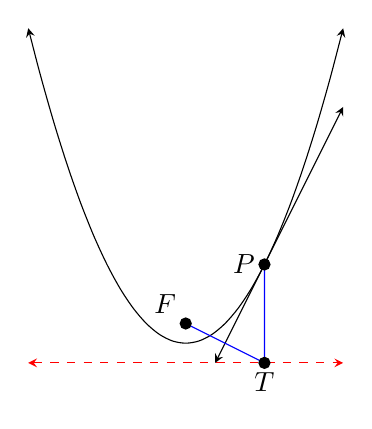
\begin{tikzpicture}[every node/.style={black}]
\draw[stealth-stealth] plot[smooth,domain=-2:2] (\x, {\x*\x});
\draw[stealth-stealth, dashed, red] (-2,-0.25) -- (2,-0.25);
\draw[stealth-stealth] (0.375,-0.25) -- (2,3);

\draw[blue] (1,1)--(1,-0.25) -- (0,0.25);

\filldraw (1,1) node[left] {$P$} circle (2pt);
\filldraw (1,-0.25) node[below] {$T$} circle (2pt);
\filldraw (0,0.25) node[above left] {$F$} circle (2pt);
\end{tikzpicture}
\end{center}

\subsubsection{Synthetic}
\begin{center}
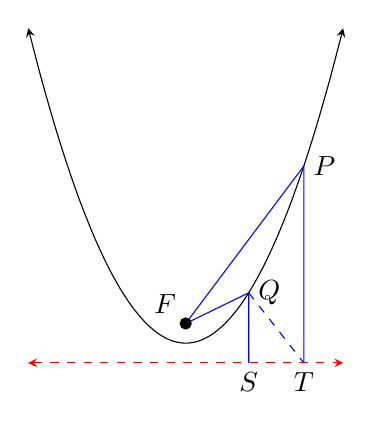
\begin{tikzpicture}[every node/.style={black}]
\draw[stealth-stealth] plot[smooth,domain=-2:2] (\x, {\x*\x});
\draw[stealth-stealth, dashed, red] (-2,-0.25) -- (2,-0.25);

\draw[blue] (0,0.25) -- (1.5,2.25) node[right] {$P$} -- (1.5,-0.25) node[below, black] {$T$};
\draw[blue] (0,0.25) -- (0.8,0.64) node[right] {$Q$} -- (0.8,-0.25) node[below, black] {$S$};
\draw[blue, dashed] (0.8,0.64) -- (1.5,-0.25);

\filldraw (0,0.25) node[above left] {$F$} circle (2pt);
\end{tikzpicture}
\end{center}
Let $F$ be the focus of the parabola,
let $P$ and $Q$ be distinct points on the parabola,
and let $T$ and $S$ be points of the directrix such that $PT$ and $QS$ are perpendicular to the directrix.
\\

By definition of a parabola $|QF|=|QS|$ and $|PF|=|PT|$,
and by construction $\triangle QST$ is a right angled triangle,
meaning:
\begin{equation*}
\begin{aligned}
|QT|^2 =& |QS|^2+|ST|^2 \\
=& |QF|^2+|ST|^2 \\
\Rightarrow |QT| >& |QF| \\
\end{aligned}
\end{equation*}

Hence the general point $Q$ isn't on the perpendicular bisector of $FT$,
but $P$ is, 
hence the perpendicular bisector of $FT$ is the tangent at $P$.

\subsubsection{Analytical}
Without loss of generality consider the unit parabola given by:
\[u: y=x^2\]
I state, without proof, that the focus is at $F=\left(0,\frac{1}{4}\right)$ and the directrix is given by:
\[d: y = -\frac{1}{4}\]
The tangent of $u$ at $P=(p,p^2)$ is given by:
\[t: y = 2px-p^2\]
Let $T=\left(p,-\frac{1}{4}\right)$ be the point of directrix such that $PT$ is perpendicular to it.
The line connecting the focus to $T$ is given by:
\[a: y= -\frac{x}{2p}+\frac{1}{4}\]
$a$ and $t$ are perpendicular since the product of their gradients is $-1$:
\[-\frac{1}{2p}\times 2p = -1\]
Also notice that the midpoint of $FT$ is given by:
\[M=\left(\frac{1}{2}(p+0),\frac{1}{2}\left(-\frac{1}{4}+\frac{1}{4}\right)\right) = \left(\frac{p}{2},0\right)\]
Is a point on both $a$ and $t$.

\subsection{Elementary Results}
\subsubsection{All points on a parabola are on the same side of the directrix as the focus:}
\begin{center}
\begin{tikzpicture}[every node/.style={black}]
	\draw[red,dashed,stealth-stealth] (-2.5,0) -- (2.5,0);
	\draw (-2,2) coordinate (F) node[above] {$F$} 
	-- (0,0) coordinate (Q) node[below] {$Q$} 
	-- (2,-2) coordinate (P) node[below] {$P$} 
	-- (2,0) coordinate (T) node[above] {$T$}
	pic[draw] {right angle = Q--T--P};
\end{tikzpicture}
\end{center}
Let $P$ be a point on the parabola on the opposite side of the focus $F$.
Let $T$ be a point on the directrix such that $PT$ is perpendicular to it.
Since $P$ and $F$ are on opposite sides of the directrix there is a point $Q$ where the segment $FP$ intersects the directrix.
\[|FP| > |QP| > |TP|\]
Which contradicts $|FP|=|TP|$,
hence $P$ doesn't exist.

\subsubsection{A line perpendicular to the directrix intersects a parabola at most once:}
\begin{center}
\begin{tikzpicture}[every node/.style={black}]
	\draw[red,dashed,stealth-stealth] (-2.5,0) -- (2.5,0);
	\coordinate (F) at (-1,3);
	\coordinate (P) at (1,4);
	\coordinate (Q) at (1,2);
	\coordinate (T) at (1,0);
	\coordinate (O) at (0,0);

	\draw (F) node[left] {$F$}
	-- (P) node[right] {$P$}
	-- (T) node[below] {$T$};

	\draw (F) -- (Q) node[right] {$Q$};

	\pic[draw] {right angle = Q--T--O};
\end{tikzpicture}
\end{center}
Let $T$ be the point where a perpendicular line to the directrix intersects the directrix.
Let $P$ and $Q$ be points on the same perpendicular line.
From the previous results both $P$ and $Q$ are on the same side as the focus $F$.
Without loss of generality let $P$ be the point further away from the directrix.
\\

Since $P$ and $Q$ are points on the parabola we have:
\[|FP| = |PT|\text{ and }|FQ| = |QT|\]
Substituting into the triangle inequality gives:
\begin{equation*}
\begin{aligned}
	|PT| =& |PQ|+|QT| \\
	=& |PQ| + |QF| \\
	>& |PF| \\
\end{aligned}
\end{equation*}
Which contradicts $|FP|=|TP|$,
hence distinct $P$ and $Q$ don't exist.

\subsubsection{A line perpendicular to the directrix intersects a parabola at least once:}
\begin{center}
\begin{tikzpicture}[every node/.style={black}]
	\draw[red,dashed,stealth-stealth] (-4.5,0) -- (2.5,0);
	\coordinate (F) at (-1,2);
	\coordinate (P) at (1,4);
	\coordinate (T) at (1,0);

	\draw (F) node[left] {$F$}
	-- (P) node[right] {$P$}
	-- (T) node[below] {$T$}
	-- (F);

	\pic[draw] {right angle = T--F--P};
\end{tikzpicture}
\end{center}
Let $F$ be the focus and let $T$ be a point on the directrix.
Extend a perpendicular line out from $T$, 
if the perpendicular intersects $F$ then the midpoint $M$ of $FT$ is on the parabola since:
\[|MF| = |MT|\]

If the perpendicular line doesn't go through $F$ suspend a second perpendicular line from the first perpendicular line at $F$ and let the two lines intersect at the point $P$.
\\

Let $X$ be a point on the segment $PT$ and define the function:
\[f(X) = |XF|-|XT|\]
We have:
\[f(T) = |TF|-|TT| > 0\]
and since $\angle PFT$ is a right angle we have $|PF| < |PT|$:
\[f(P) = |PF|-|PT| < |PT| -|PT| = 0\]
Hence by continuity there is a point $X_0$ in the segment $PT$ such that:
\[f(X_0) = 0\]
Meaning:
\[|X_0F| = |X_0T|\]
As required.

\subsubsection{A line perpendicular to the directrix intersects a parabola exactly once:}
Combine the last two results.

\subsubsection{Remarks}
These arguments are non-euclidean in two senses.
Neither sense as cool as "non-euclidean" sounds,
both of them still interesting.
\\

Firstly, is the use of continuity in the penultimate result.
The euclidean axioms famously don't include a concept of continuity.
Adding a continuity axiom to Euclid and when the concept is implicitly used has been an ongoing topic of research since the 19th century.
\\

Secondly, is the reverse.
Instead of using an another one,
we might not need to use all the euclidean axioms.
The first results don't use right-angles beyond showing $|PQ| > |PT|$ and the second result doesn't use them at all.
To me, this suggests that these results can be generalized to some subset of euclidean geometry.
I wasn't able to do so here,
but thoughts like this are why I wanted to think about parabolas more.

%% An unused diagram I don't feel like deleting.
%
%\begin{center}
%\begin{tikzpicture}[every node/.style={black}]
%	\coordinate (F) at (-2,0);
%	\coordinate (P) at (0,2);
%	\coordinate (Q) at (0,-2);
%	\coordinate (T) at (2,0);
%
%	\draw (F) node[left] {$F$} 
%	-- (P) node[above] {$P$}
%	-- (T) node[right] {$T$}
%	-- (Q) node[below] {$Q$}
%	-- (F);
%
%	\draw[red,dashed] (P) -- (Q);
%\end{tikzpicture}
%\end{center}
%With $P$ and $Q$ distinct points such that:
%\[|PT| = |PF| \text{ and } |QT| = |QF|\]
%This follows from the substitution into the triangle inequality:
%\[|PT| < |PQ|+|QT|\]
%Giving:
%\[|PT| < |PQ|+|QF|\]

%% An unused parts of an argument attempting to avoid right angles in the first result
%
%Let $F$ be the focus $P$ be the point $Q$ the intersection and $T$ the minimizing point on the directrix.
%
% Assume $|FQ| > |QT|$ then:
%\[|FP| \geq  |FQ|+|QP| > |QT|+|QP| > |TP|\]
%
%We also have:
%\[|FT|+|TP| > |FP| \geq |FQ|+|QP| = |TQ|+|QP| \geq |TP| \]


\end{document}
